% ****** Start of file apssamp.tex ******
%
%   This file is part of the APS files in the REVTeX 4.2 distribution.
%   Version 4.2a of REVTeX, December 2014
%
%   Copyright (c) 2014 The American Physical Society.
%
\documentclass[reprint,amsmath,amssymb]{revtex4-2}

\usepackage{graphicx}% Include figure files
\usepackage{dcolumn}% Align table columns on decimal point
\usepackage{bm}% bold math
\usepackage{physics}
\usepackage{float}
\usepackage{listings}
\usepackage{xcolor}
\usepackage{blindtext}

\definecolor{codegreen}{rgb}{0,0.6,0}
\definecolor{codegray}{rgb}{0.5,0.5,0.5}
\definecolor{codepurple}{rgb}{0.58,0,0.82}
\definecolor{backcolour}{rgb}{0.95,0.95,0.92}

\lstdefinestyle{mystyle}{
    backgroundcolor=\color{backcolour},   
    commentstyle=\color{codegreen},
    keywordstyle=\color{magenta},
    numberstyle=\tiny\color{codegray},
    stringstyle=\color{codepurple},
    basicstyle=\ttfamily\footnotesize,
    breakatwhitespace=false,         
    breaklines=true,                 
    captionpos=b,                    
    keepspaces=true,                 
    numbers=left,                    
    numbersep=5pt,                  
    showspaces=false,                
    showstringspaces=false,
    showtabs=false,                  
    tabsize=2
}

\lstset{style=mystyle}

\begin{document}

%\preprint{APS/123-QED}

\title{Resource-Efficient Discrete Fourier Transform via the Goertzel Algorithm for Continuous Wave Detection with FPGAs}
\thanks{Algorithm first described by Gerald Goertzel, 1958}%

\author{Connor Fricke}
\affiliation{%
 Ohio State University, Center for Cosmology and Astroparticle Physics
}%

\collaboration{CoRaLS} \noaffiliation

\date{\today}% It is always \today, today,

\begin{abstract}
In many \textit{digital signal processing} (DSP) applications, the \textit{Discrete Fourier Transform} (DFT) is used as a method of breaking down a signal into its corresponding frequency components. It is a conversion of a discretized finite-duration signal from the time domain into the frequency domain, producing a discrete \textit{power spectrum}. A \textit{field-programmable gate-array} (FPGA) is a computer chip designed with reconfigurable ("field-programmable") internal logic allowing for a wide range of applications---often used to avoid expensive and inflexible specialized hardware. FPGAs lend themselves to signal processing applications because of their capabilities for parallel mathematical operations such as digital filters. Standard \textit{fast Fourier transform} (FFT) algorithms often require more FPGA resources than is desirable. The \textit{Goertzel algorithm} presents as an alternative, allowing the DFT to be casted as a type of digital filter which determines the Fourier coefficient of a single frequency. In some applications this "single-tone" DFT may not be entirely useful; however, the system benefits greatly from the filter's minimized usage of logic elements such as registers, multipliers, and accumulators; in other words, the filter's \textit{"hardware footprint"} is far smaller than commonly used FFT alternatives.
\begin{description}
\item[Keywords]
Field-Programmable Gate Array (FPGA), Digital Signal Processing (DSP),\\ Digital Filters, Goertzel Algorithm, Discrete Fourier Transform (DFT)
\end{description}
\end{abstract}

\maketitle

\section{Background}

In many astrophysics and astronomy experiments such as the \textit{Antarctic Impulsive Transient Antenna} (ANITA) and its successor, the \textit{Payload for Ultrahigh Energy Observations} (PUEO), researchers indirectly study astrophysical processes via detection and observation of their byproducts. In the case of ANITA and PUEO, a radio-frequency (RF) impulsive signal is generated via the \textit{Askaryan effect}: a process which follows the emission of \textit{Cherenkov radiation} emitted by the collision interaction of cosmic neutrinos within water-ice. Neutrinos are famously elusive particles to detect, as they are low mass particles with no electrical charge, and thus neutrinos only rarely interact with matter. For this reason, the aim of projects like ANITA and PUEO which seek to detect them (or rather, the byproducts of their interactions with matter) must maximize the duration, resolution, and bandwidth of their observations. In turn, this elicits extremely large amounts of incoming data that must be processed very quickly and efficiently before it is stored or erased, thus FPGAs are heavily involved in the data acquisition stage of such experiments.

As is inherent of all upper atmosphere and outer space experiments, cosmic radiation poses a severe threat to the integrity of gathered data as well as the hardware which processes it. \textit{Single-event upsets} (SEU) occur when a singular ionizing particle such as a cosmic ray interferes with internal logic in an operating electronic device such as a memory block, integrated circuit, or ADC. An SEU is likely to disrupt the behavior of ongoing mathematical processes which may seem to result in a "scrambling" of data or other incorrect observations. In general, methods designed to detect, reduce, or prevent the effects of ionizing radiation are referred to as \textit{radiation hardening}.

An implementation of the Goertzel algorithm---more generally, any form of DFT---inside an FPGA could theoretically behave as a form of radiation hardening for an important hardware component, the \textit{analog-to-digital converter} (ADC). Via constant frequency-domain analysis of a controlled external signal fed through an ADC, an SEU would be easily recognizable from one or more unexpected values in the resulting power spectrum. Because the Goertzel filter isolates the Fourier coefficient present in a signal for one singular frequency value, an input signal to the algorithm could be chosen such that only one or a few frequencies must be analyzed for validation of the ADC behavior. As discussed later, this control over an input signal allows for significant simplification of the algorithm, which further reduces the minimum resource requirements. In summary, the Goertzel filter ensures the integrity of concurrent ADC data by consistent detection of an expected frequency while consuming minimal hardware resources.

\section{Methods of Digital Signal Processing}

Digital signal processing is studied and applied heavily in telecommunications, defense, image processing, healthcare, scientific research, and more. The primary focus of DSP is simply the manipulation, analysis, and transformation of signals which have been digitized. A \textit{digital} signal implies a signal which is \textit{finite-duration}, \textit{discrete}, and \textit{quantized}. A discrete signal is one which has equally spaced samples taken at a finite \textit{sampling rate}. A quantized signal is one of which sample values can only take on a finite number of values---an inherent property of the binary logic in FPGAs and other processors. A digital signal can be represented very simply as a sequence of numbers, $x(n)$, with an implicit discretization and quantization of the sequence values.

\begin{figure}
    \centering
    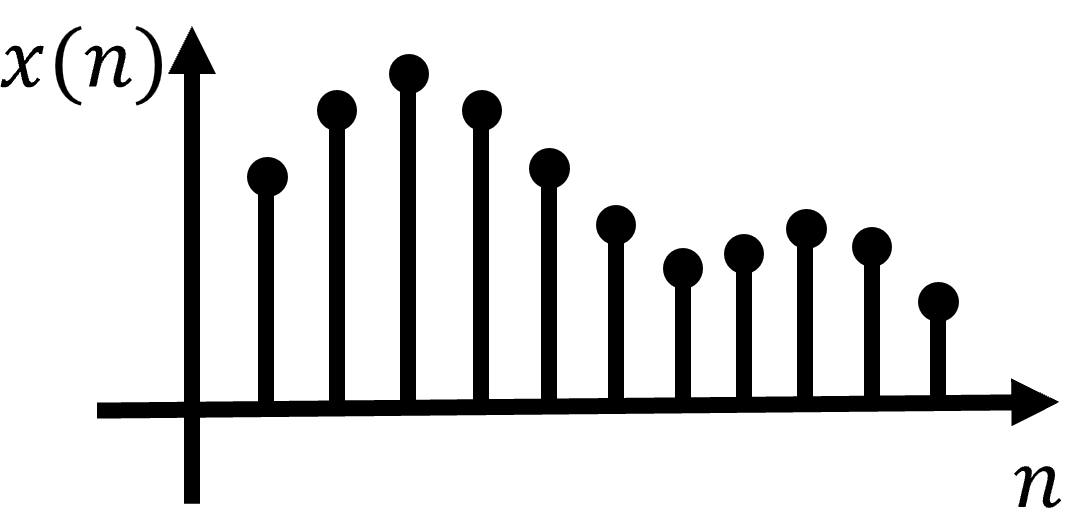
\includegraphics[width=0.6\linewidth]{figs/digital_signal.png}
    \caption{A digital signal with sample number, $n$, on the horizontal axis.}
    \label{fig:1}
\end{figure}
\begin{figure}
    \centering
    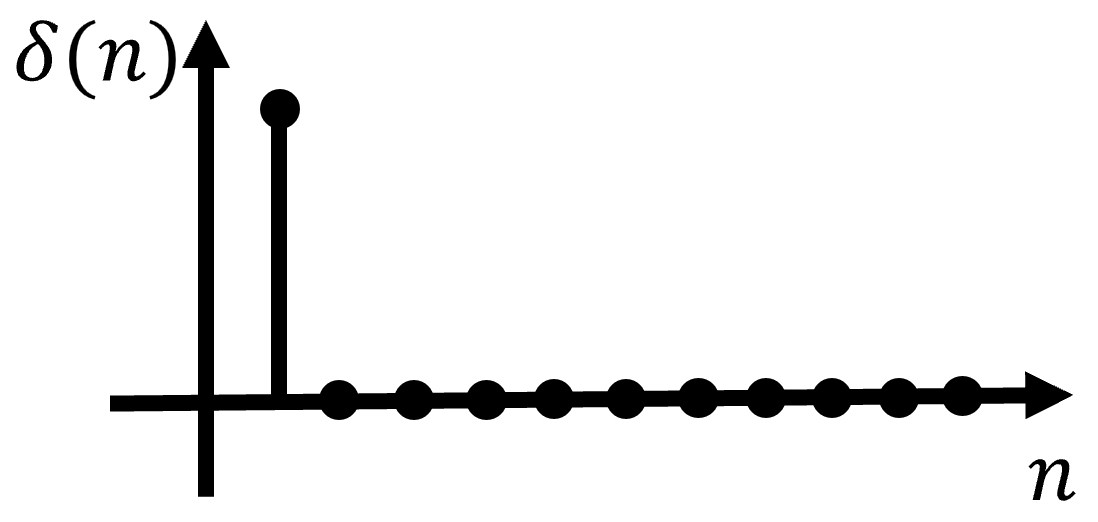
\includegraphics[width=0.6\linewidth]{figs/impulse.png}
    \caption{An impulsive signal, $\delta(n)$. Often used to characterize a digital filter via its impulse-response $h(n)$}
    \label{fig:2}
\end{figure}

\subsection{Digital Filters}

Digital filters and filter design make up their own branch of study within signal processing. They are useful for many applications, e.g., eliminating aliasing, reducing signal noise, or calculating moving averages. A \textit{system} is any mathematical transformation or operation that acts on an input sequence and returns an output sequence. Digital filters are a subclass of systems which are \textit{linear shift-invariant} (LSI). Linear systems require that the operation of the system, $T$, follows

\begin{align*}
    T[a x_1(n) + b x_2(n)] & = a T[x_1(n)] + b T[x_2(n)] \\
    & = a y_1(n) + b y_2(n) 
\end{align*}
while shift-invariance implies that if $T[x(n)] = y(n)$ then
$$
T[x(n-k)] = y(n-k)
$$
For LSI systems, the output sequence, $y(n)$, of a digital filter in response to an input sequence, $x(n)$, is given by the convolution sum,
\begin{equation}
    y(n) = \sum_{k=0}^{\infty}x(k)\cdot h(n-k)
\end{equation}
where the \textit{impulse response}, $h(n)$, is the response of the filter to an impulsive signal. All digital filters can be characterized by their impulse response. Filters can be divided into two groups, referred to as \textit{finite-duration impulse-response} (FIR) and \textit{infinite-duration impulse-response} (IIR). Generally, IIR filters have output sequence values which depend on previous \textit{output} values, while an FIR filter output depends only on previous \textit{inputs}. A particular filter may belong to one or both of these classes.

It is often necessary to impose further constraints that the system must be both \textit{causal} and \textit{stable}. A causal filter requires that all outputs of the system depend only on the current or previous inputs or outputs, not future ones. This is a requirement of implementing the filter in hardware (input/output values cannot be used before you obtain them). A stable filter is one for which the impulse response of the filter converges to zero. More formally,
\begin{align*}
    h(n) = 0 \text{ if } n < 0 \ \ \ \ \ & \text{(causal)} \nonumber \\
   \sum_{k=-\infty}^\infty{\abs{h(k)}} < \infty \ \ \ \ & \text{(stable)} \nonumber
\end{align*}

An FPGA implementation of the Goertzel filter should attain both stability and causality. (See Ref. \cite{DSP}).

\subsection{Difference Equations}

Another method of characterizing digital filters is through their difference equations. For linear shift-invariant systems, it is useful to demonstrate the behavior using the filter's \textit{linear constant-coefficient difference equation},
\begin{equation}
    \sum_{k=0}^Na_ky(n-k) = \sum_{r=0}^Mb_rx(n-r)
\end{equation}

These difference equations illustrate a more straightforward mathematical approach to implementing a particular filter. As an example, it would be quite simple to calculate an output sequence from a filter described by the difference equation
$$
y(n) = \alpha \cdot x(n) + (1-\alpha)\cdot y(n-1)
$$
where $x(n)$ and $y(n)$ are the $n$-th system input and output values, respectively. Difference equations are an equivalent method to the impulse-response method of characterizing digital filters as evidenced by the convolution (denoted by $*$) relationship between the filter's output, input, and impulse response: (See Ref. \cite{DSP}).
\begin{equation}
    y(n) = h(n) * x(n)
\end{equation}
In addition, this relationship extends to the complex z-plane, as discussed in the next section.

\subsection{The z-Transform}

\begin{figure}
    \centering
    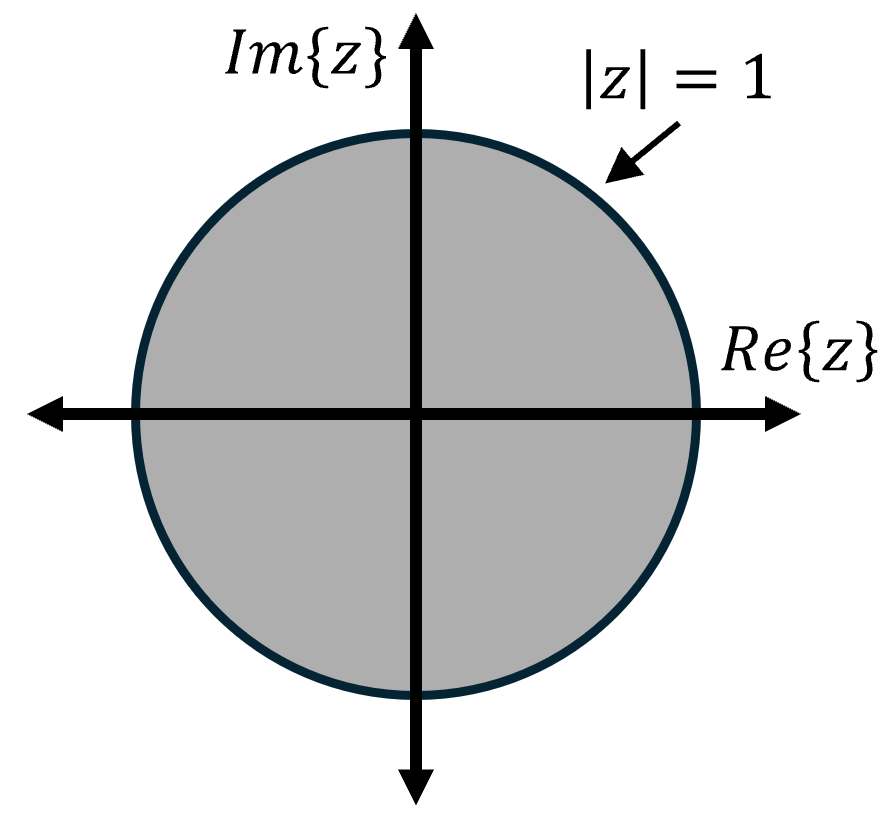
\includegraphics[width=0.6\linewidth]{figs/zplane.png}
    \caption{The complex-valued z-plane. Stable filters require that all poles of the transfer function are within the unit circle.}
    \label{fig:3}
\end{figure}

It is quite common when working with digital filters to use the complex z-plane for further characterization as well as studying filter behavior. The z-transform is defined as
\begin{equation}
    X(z) = \sum_{n=0}^\infty x(n)\cdot z^{-n}
\end{equation}
where $z$ is a complex number, and $x(n)$ is a discrete input sequence. The z-plane representation of a digital filter follows quite simply as the z-transform of the filter's impulse response,
\begin{equation}
    H(z) = \sum_{n=0}^\infty h(n)\cdot z^{-n}
\end{equation}

This is is often referred to as the \textit{system function} or \textit{transfer function} of the filter. All filters have transfer functions which can be represented as a ratio of polynomials in $z$. From this representation, it is easy to locate the poles and zeros of the transfer function, which are points of interest in designing digital filters.
\begin{equation}
    H(z) = \frac{1+\beta_1z^{-1} + \ldots + \beta_Mz^{-M}}{1+\alpha_1z^{-1} + \ldots + \alpha_Nz^{-N}}
\end{equation}

Pole-zero analysis is an important part of designing and understanding any filter. For example, a filter is known to be stable if and only if all of its poles are inside the unit circle of the z-plane.

An important mathematical property of the z-transform is its convolution property, which states that the z-transform of a convolution of two sequences $Z[x_1(n)*x_2(n)]$, is equivalent to the product of each sequence's z-plane representation, $X_1(z)\cdot X_2(z)$. More importantly, this demonstrates a relationship between filter behavior and the z-plane.
\begin{equation}
    Z[x(n)*h(n)] = X(z)\cdot H(z) \nonumber
\end{equation}
where $y(n) = x(n) * h(n)$, therefore
\begin{equation}
    Y(z) = X(z) \cdot H(z) 
\end{equation}
and so a new definition of the transfer function is obtained.
\begin{equation}
    H(z) = \frac{Y(z)}{X(z)}
\end{equation}

\subsection{Fourier Transforms}

Another useful tool among those available in signal processing is the well-known \textit{Fourier transform}. It serves as a formula for converting any function, $f(t)$, from its time-domain representation to an equivalent frequency representation, $f(\omega)$. The normalized values of the function $f(\omega)$ represent the coefficients of the infinite \textit{Fourier series} for all possible frequencies, $\omega$. As a result, the Fourier transform provides a straightforward way of analyzing the continuous wave frequencies which are present in any real or complex signal. For continuous functions, the Fourier transform is defined as an integral.
\begin{equation}
    f(\omega) = \int_{-\infty}^\infty f(t)\cdot e^{-i2\pi\omega t} \,dt 
\end{equation}

However, a digital signal is neither continuous nor is it infinite in duration like the function $f(t)$ in the integrand of the Fourier transform. Without going into the various methods or interpretations of the derivation of the \textit{Discrete Fourier Transform}, its relationship with the continuous Fourier transform is fairly obvious. The DFT is defined:
\begin{equation}
    X(k) = \sum_{n=0}^{N-1}{x(n)\cdot e^{-i2\pi kn/N}}
\end{equation}

In this definition, a few notable changes have occurred. Of course, the continuous form's independent variable, $t$, is now represented as $n$, which corresponds to the sample number in the discretized sequence. The sum has constrained bounds due to a finite number of values available in the input sequence, $x(n)$. It should also be noted that the continuous-valued frequency, $\omega$, is replaced with $k/N$, which suggests a relationship between the \textit{integer}-valued $k$ and the sequence length, $N$. Though there are many interpretations, the most important takeaway is that k represents some scaled frequency. Its relationship with a real frequency (measured in Hz) is discussed later. 

Importantly, this form of the DFT is \textit{unnormalized}, since normalization would mean a factor of $\frac{1}{N}$ in front of the sum in equation \textbf{(10)}. If single $k$-frequency with an amplitude of unity is present, then the resulting $|X(k)|$ should be $N/2$. The reason it is not $N$ is because the DFT is often (by convention) calculated and normalized over the range from negative to positive \textit{Nyquist}, $-N/2$ to $N/2$. For a real valued signal like a sine wave, the remaining amplitude of the result is present at $|X(-k)|$ since negative and positive frequencies are indistinguishable.

\section{The Goertzel Algorithm}

Now that some important tools of signal processing (filters, filter responses, transfer functions, transforms) have been laid out, the \textit{Goertzel algorithm} is within reach. The goal of the Goertzel algorithm is an alternative mathematical approach to performing the DFT. First, recall the definition of the DFT,
$$
    X(k) = \sum_{n=0}^{N-1}{x(n)\cdot W_N^{kn}}
$$
where $W_N^{kn} = e^{-i2\pi kn/N}$ for integer values of $k$. Importantly, $W_N^{-kN} = e^{i2\pi k} = 1$ regardless of $k$, and so multiplying the DFT sum by $W_N^{-kN}$ does not change the result. The new DFT definition becomes
\begin{align}
    X(k) & = W_N^{-kN} \sum_{n=0}^{N-1}{x(n)\cdot W_N^{kn}}\nonumber \\
         & = \sum_{n=0}^{N-1}{x(n)\cdot W_N^{-k(N-n)}}
\end{align}
Evidently, this definition is a discrete convolution sum of $x(n)$ with another sequence $W_N^{-kn} = e^{i2\pi kn/N}$. Recall that in general, the output of any filter is simply the convolution of an input sequence, $x(n)$, with the filter's impulse response, $h(n)$. Any filter characterized by 
\begin{equation}
    h(n) = W_N^{-kn} = e^{i2\pi kn/N}
\end{equation}
 will then yield an output sequence for a fixed value of $k$ with the convolution sum,
 \begin{equation}
     y_k(n) = \sum_{r=0}^{N-1}{x(r)\cdot W_N^{-k(n-r)}}
 \end{equation}
 and thus the result of the DFT is given by the N-th value of this output sequence (see Ref. \cite{DSP}).
 \begin{align}
     X(k) & = y_k(n)|_{n=N} 
    \nonumber \\
     & = \sum_{r=0}^{N-1}{x(r)\cdot W_N^{-k(N-r)}}
 \end{align}

\subsection{First-Order Goertzel Filter}

\begin{figure}
    \centering
    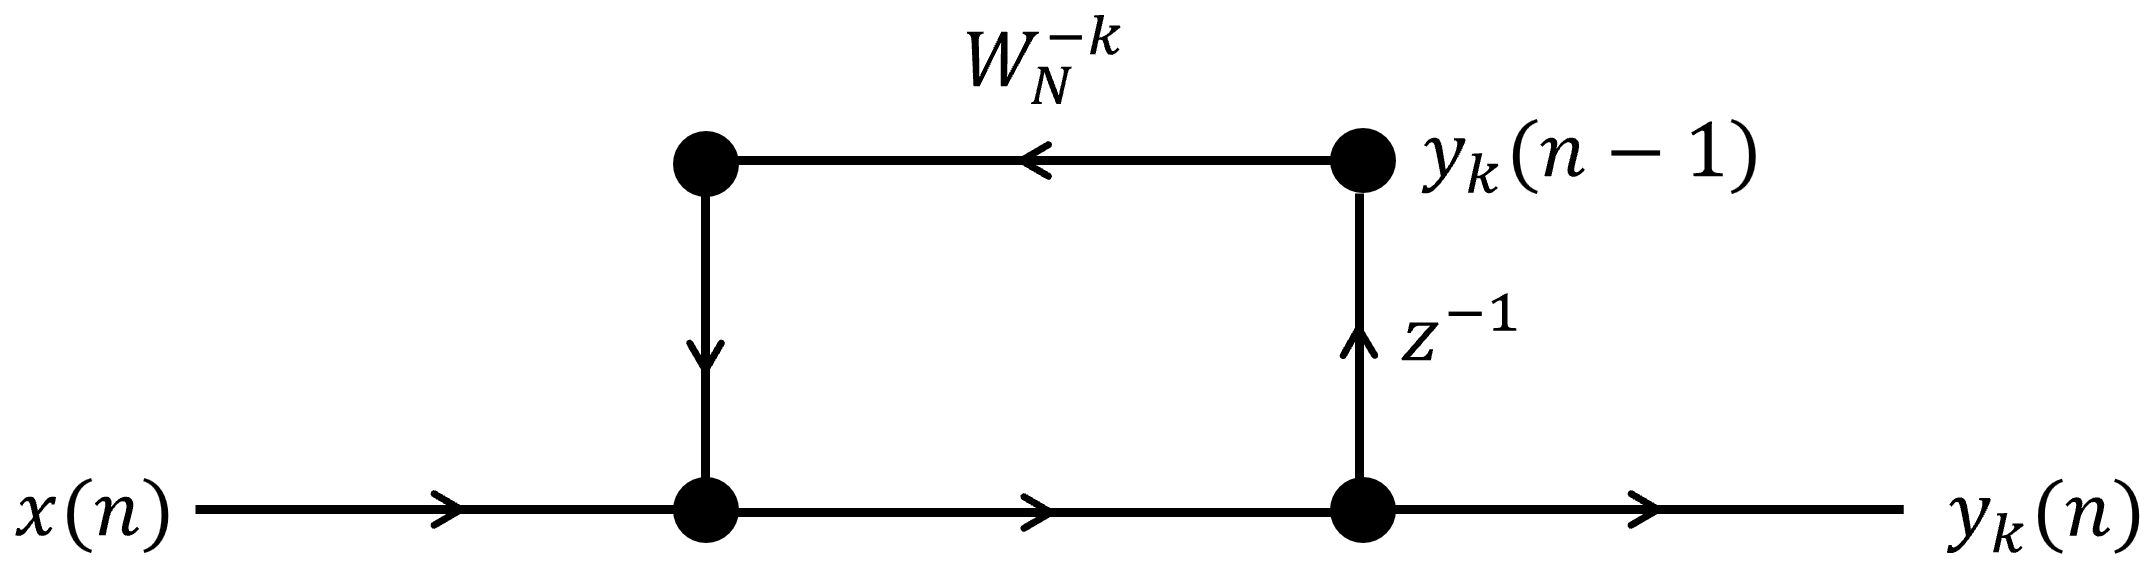
\includegraphics[width=\linewidth]{figs/goertzel_network1.png}
    \caption{First-order signal flow graph of the Goertzel filter}
    \label{fig:4}
\end{figure}

\textbf{FIG. 4} shows the network representation of the first-order Goertzel filter designed to implement the convolution given by equations \textbf{(11)} and \textbf{(14)}. The nodes and arrows in the network are representations of the flow of data through a filter in such a way that highlights the structure of a hardware implementation. An arrow with a value nearby implies the value being multiplied by the constant as it passes through to the next node. Any node where arrows meet implies a summation of the incoming values. Because of the implicit relationship of filters with the z-plane and z-transform, a multiplication by a factor of $z^{-1}$ represents a \textit{unit delay}, meaning a signal is delayed by one sample. A unit delay of $y_k(n)$ in this network results in $y_k(n-1)$ stored at the node above.

The difference equation of the \textit{first-order Goertzel filter} is
\begin{equation}
    y_k(n) = x(n) + W_N^{-k}\cdot y_k(n-1)
\end{equation}
which, via z-transform, corresponds to a transfer function,
\begin{equation}
    H_k(z) = \frac{Y_k(z)}{X(z)} = \frac{1}{1-W_N^{-k}z^{-1}}
\end{equation}

Evidently, from the \textit{feedback loop} in the network of \textbf{FIG. 4}, the $y_k(n-1)$ term in equation \textbf{(15)}, and the structure of equation \textbf{(16)}, the first-order filter is purely IIR. Both the input and output are complex-numbered sequences, thus each output value calculated requires 4 real additions and 4 real multiplications. Since computing $X(k)$ requires carrying out the entire filter process from $y_k(0)$ to $y_k(N)$, the entire algorithm takes a minimum of $4N$ real additions and $4N$ real multiplications for a single $k$ value.

\subsection{Second-Order Goertzel Filter}

\begin{figure*}
    \centering
    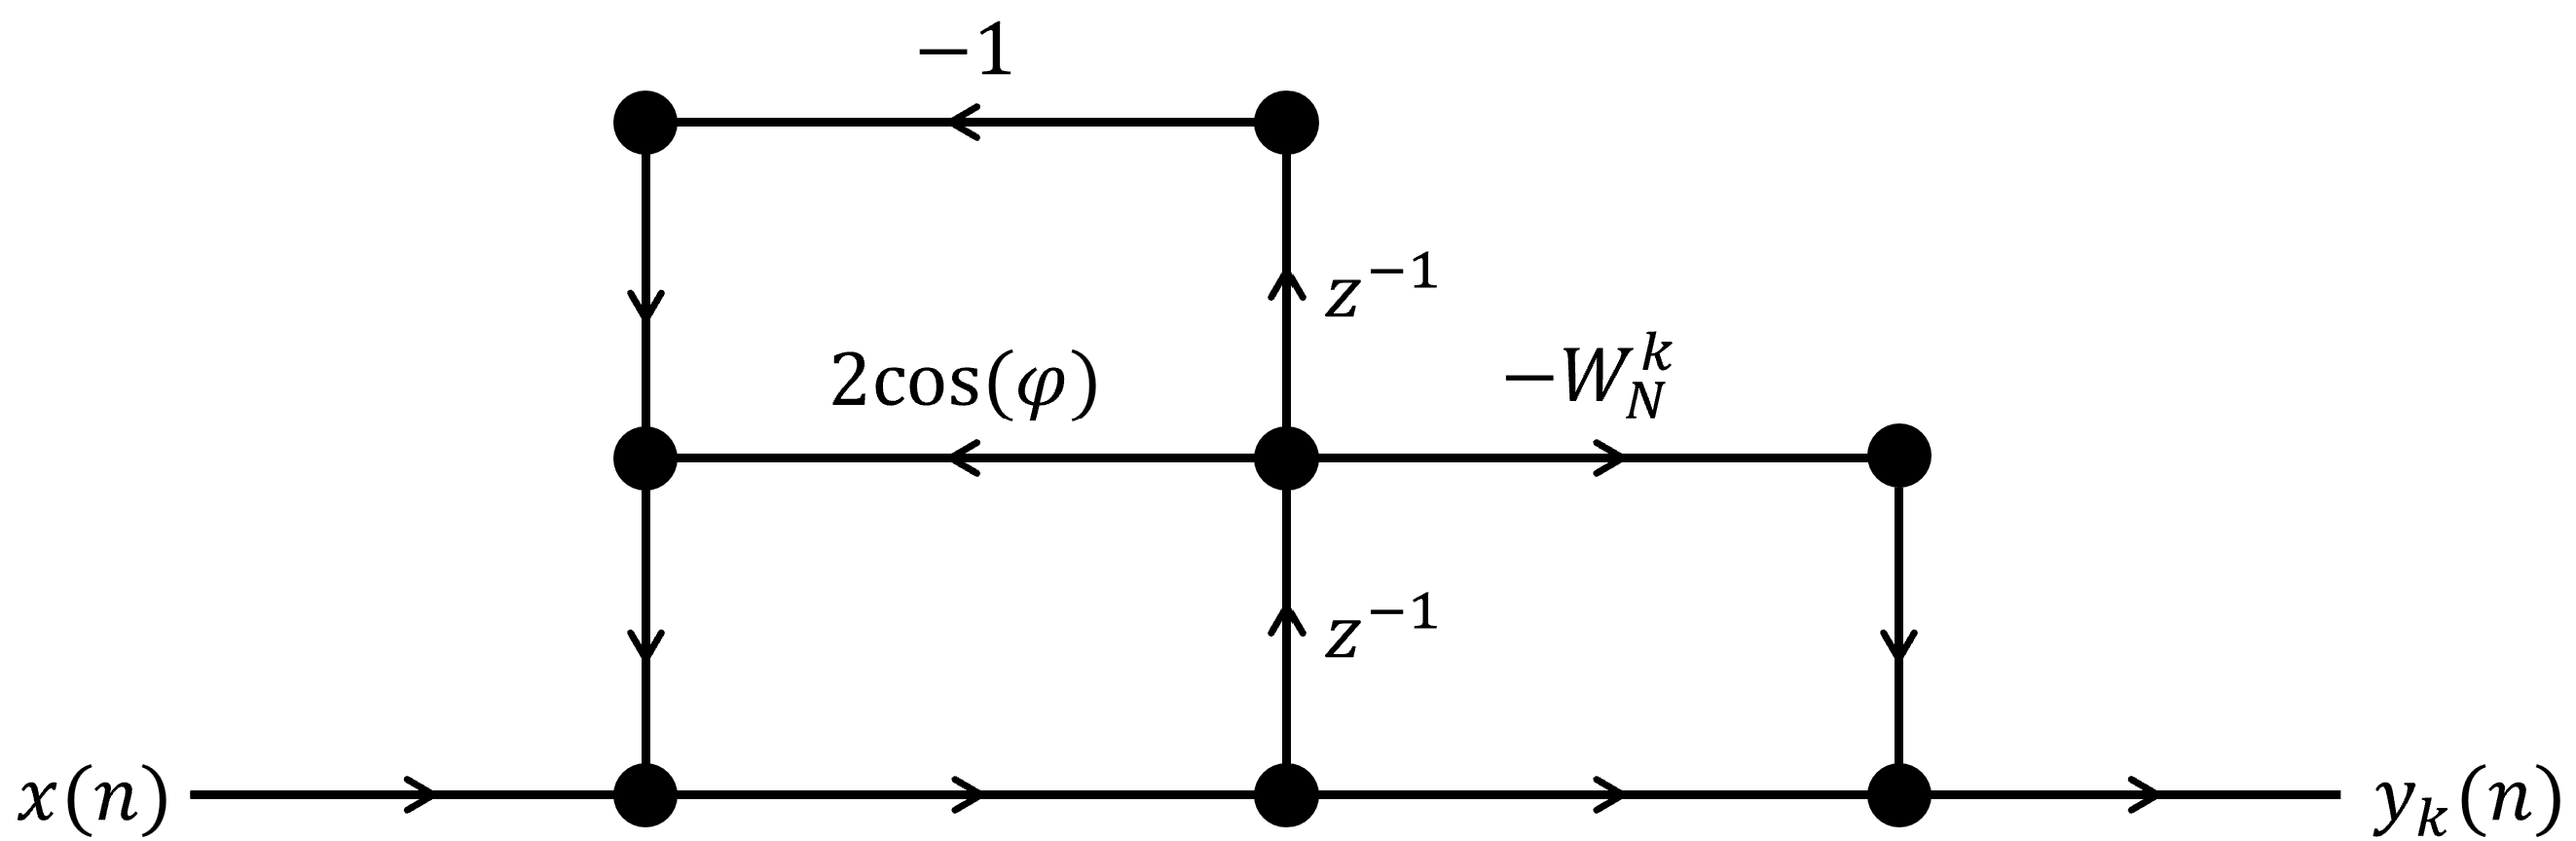
\includegraphics[width=0.7\linewidth]{figs/goertzel_network2.png}
    \caption{Second-order Goertzel filter signal flow graph}
    \label{fig:5}
\end{figure*}

\begin{figure*}
    \centering
    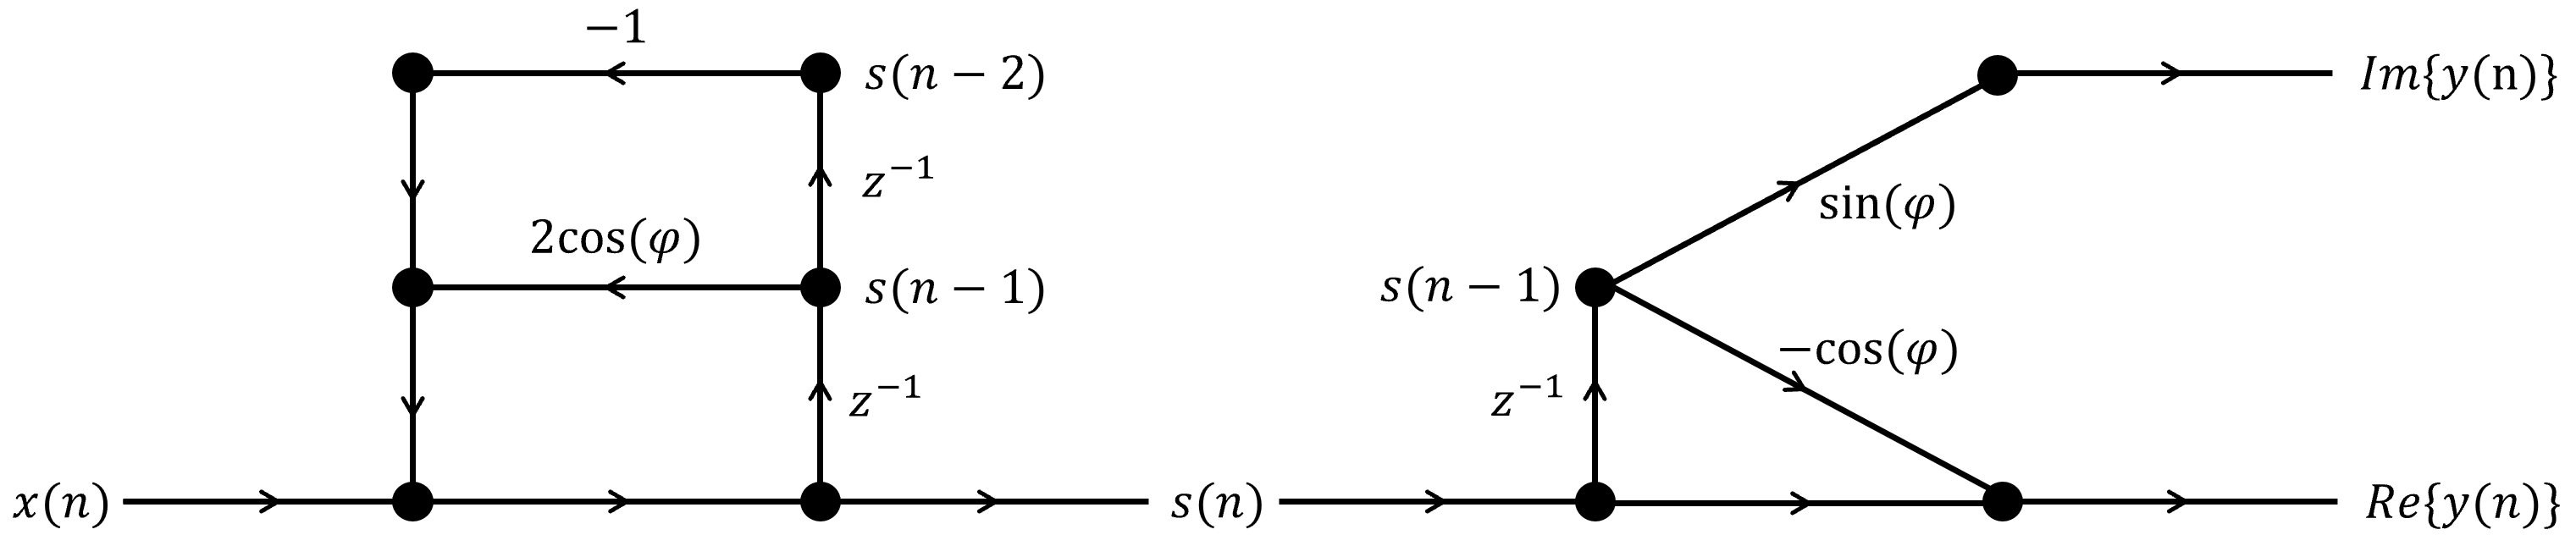
\includegraphics[width=\linewidth]{figs/goertzel_cascade.png}
    \caption{Second-order Goertzel filter signal flow graph, cascade form with explicit real and imaginary calculation}
    \label{fig:6}
\end{figure*}

By multiplying the numerator and denominator of the first-order transfer function by $(1-W_N^kz^{-1})$, the filter takes on a different form. The \textit{second-order Goertzel filter} has both FIR and IIR components.
\begin{align}
    H_k(z) & = \frac{1}{1-W_N^{-k}z^{-1}} \nonumber \\
           & = \frac{1}{1-W_N^{-k}z^{-1}} \frac{(1-W_N^kz^{-1})}{(1-W_N^kz^{-1})} \nonumber \\
           & = \frac{1-W_N^kz^{-1}}{1-2\cos(2\pi k/N)z^{-1} + z^{-2}}
\end{align}
At first, the second-order form may seem more complex, however this implementation reduces the number of multiplications by roughly a factor of two. The difference equation follows as
\begin{align}
    y_k(n) & = x(n) - W_N^k\cdot x(n-1) \ldots \nonumber \\ & +\ 2\cos(\varphi)\cdot y(n-1) - y(n-2)
\end{align}
where $\bm{\varphi = 2\pi k/N}$. In order to implement the poles (the IIR portion) of the filter, only two real multiplications, namely $2\cos(\varphi)\cdot \Re{y(n-1)}$ and $2\cos(\varphi)\cdot \Im{y(n-1)}$, are required for each sample, as well as four real additions. The signal flow graph of this new form is illustrated in \textbf{FIG. 5}.

The FIR portion of the filter (the \textit{feedforward loop} within the signal flow diagram) can be isolated from the IIR component. It is useful to define an intermediate sequence, $s(n)$, as the result of the initial IIR filter pass on the input sequence. The resulting difference equations are
\begin{align}
    s(n) & = x(n) + 2\cos(\varphi)\cdot s(n-1) - s(n-2) \\
    y_k(n) & = s(n) - W_N^k\cdot s(n-1)
\end{align}

In this case, the IIR component can be implemented separately, while the effects of the FIR component can be appended at the final step of the process with only four more multiplications and four more additions since the FIR output depends solely on $s(N)$ and $s(N-1)$. In total, the second-order form of the Goertzel algorithm requires $2(N + 2)$ multiplications and $4(N+1)$ additions for a single $X(k)$ calculation.

\textbf{FIG. 6} highlights the multi-step process of this \textit{cascade form}. Note that the multiplication by the complex coefficient has been split into its real and imaginary components, as is necessary for an implementation in software (a \textit{C++} program, for example) or hardware (FPGA).

\subsection{Signal Extension}

It is important to note that by definition, the DFT requires $N$ terms ($n=0$ to $n=N-1$) to perform the full calculation. The implementation of the Goertzel filter, however, requires $N+1$ samples for its calculation, since $X(k)$ is the $(N+1)$-th term of the output sequence, $y_k(n)|_{n=N}$. The workaround to this is quite simple. Append an extra term to the input sequence, $x(N) = 0$. By assuming the presence of this extra sample in the input sequence, the last required term of the intermediate sequence follows from equation \textbf{(19)}, 
\begin{equation}
    s(N) = 2\cos(\varphi)\cdot s(N-1) - s(N-2)
\end{equation}
which can then be used in the final step: 
\begin{align}
    X(k) & = y_k(n)|_{n=N} \\
    & = s(N) - W_N^k\cdot s(N-1) \nonumber \\
    & = [2\cos(\varphi) s(N-1) - s(N-2)] - W_N^k\cdot s(N-1)  \nonumber \\
    & = W_N^{-k}\cdot s(N-1) - s(N-2) \nonumber
\end{align}


\section{Software Implementation}

\begin{figure*}
    \centering
    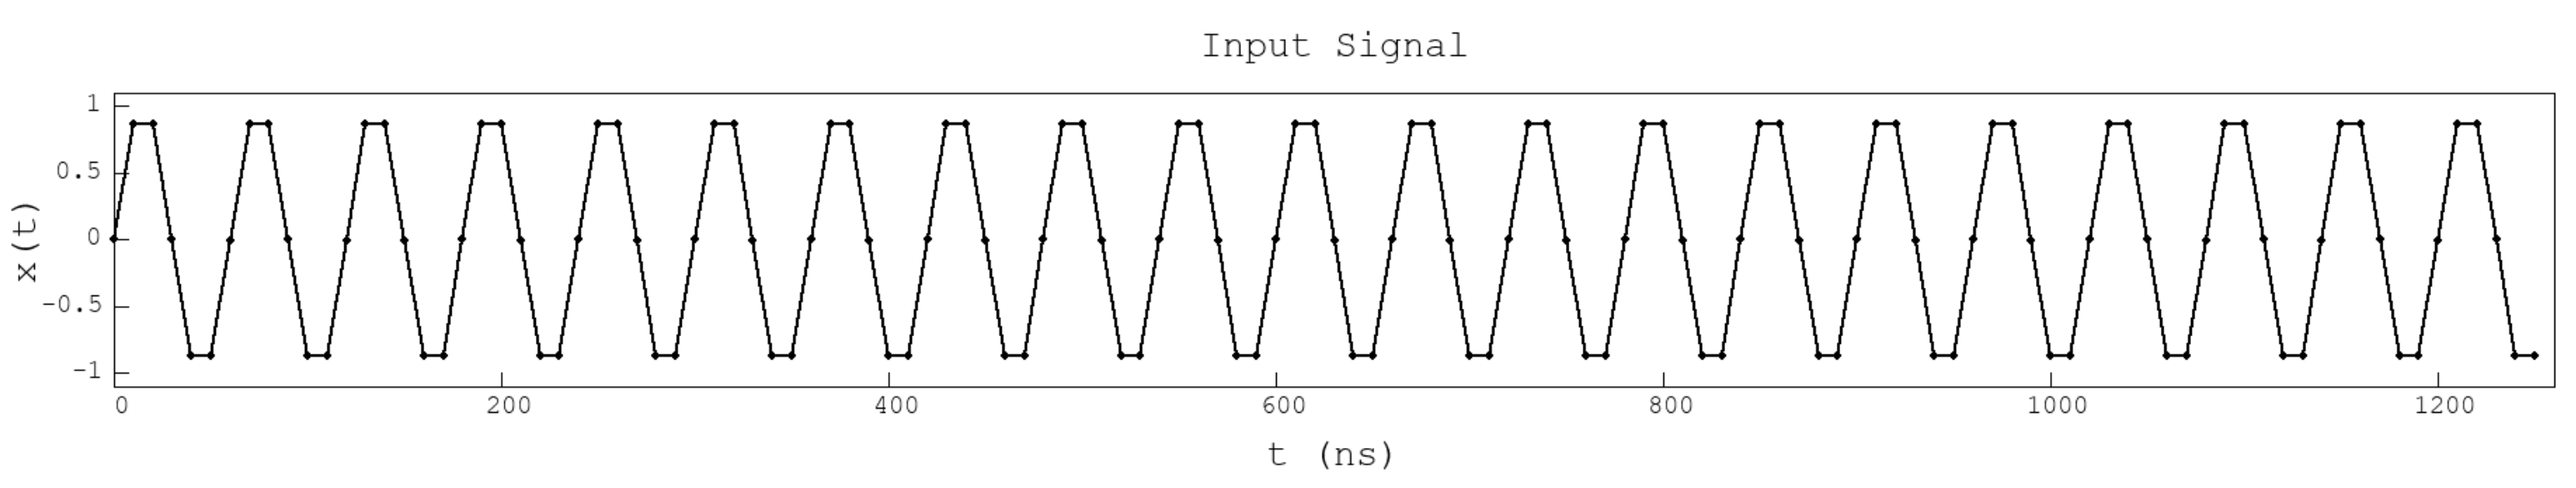
\includegraphics[width=\linewidth]{figs/sine_signal.png}
    \caption{\textit{C++} generated signal, $x[n]$ with sampling frequency, $f_s = 100$ MHz, signal frequency, $f = f_s/6 = 16.67$ MHz, and $N = 126$. An unnormalized DFT should yield $|X(k)| = 63$ for the corresponding $k$ value  (See Ref. \cite{github}).}
    \label{fig:7}
\end{figure*}

\begin{figure*}
    \centering
    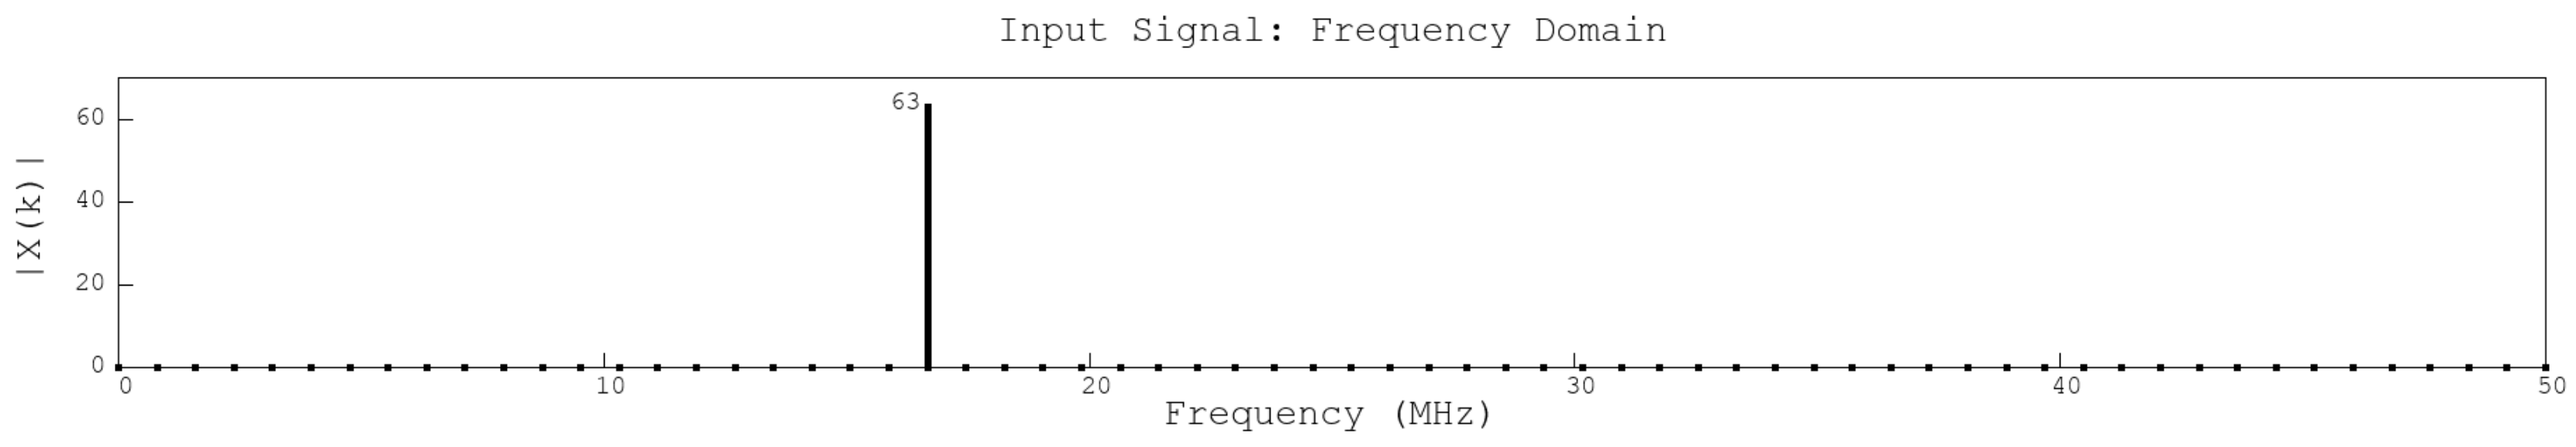
\includegraphics[width=1.01\linewidth]{figs/signal_DFT.png}
        \caption{DFT results for integer $k$ values over the interval $[0,\frac{N}{2}]$, given sampling frequency $f_s = 100$ MHz. Transform performed via \textit{C++} implementation of the Goertzel algorithm. (See Ref. \cite{github}).}
    \label{fig:8}
\end{figure*}

\begin{figure*}
    \centering
    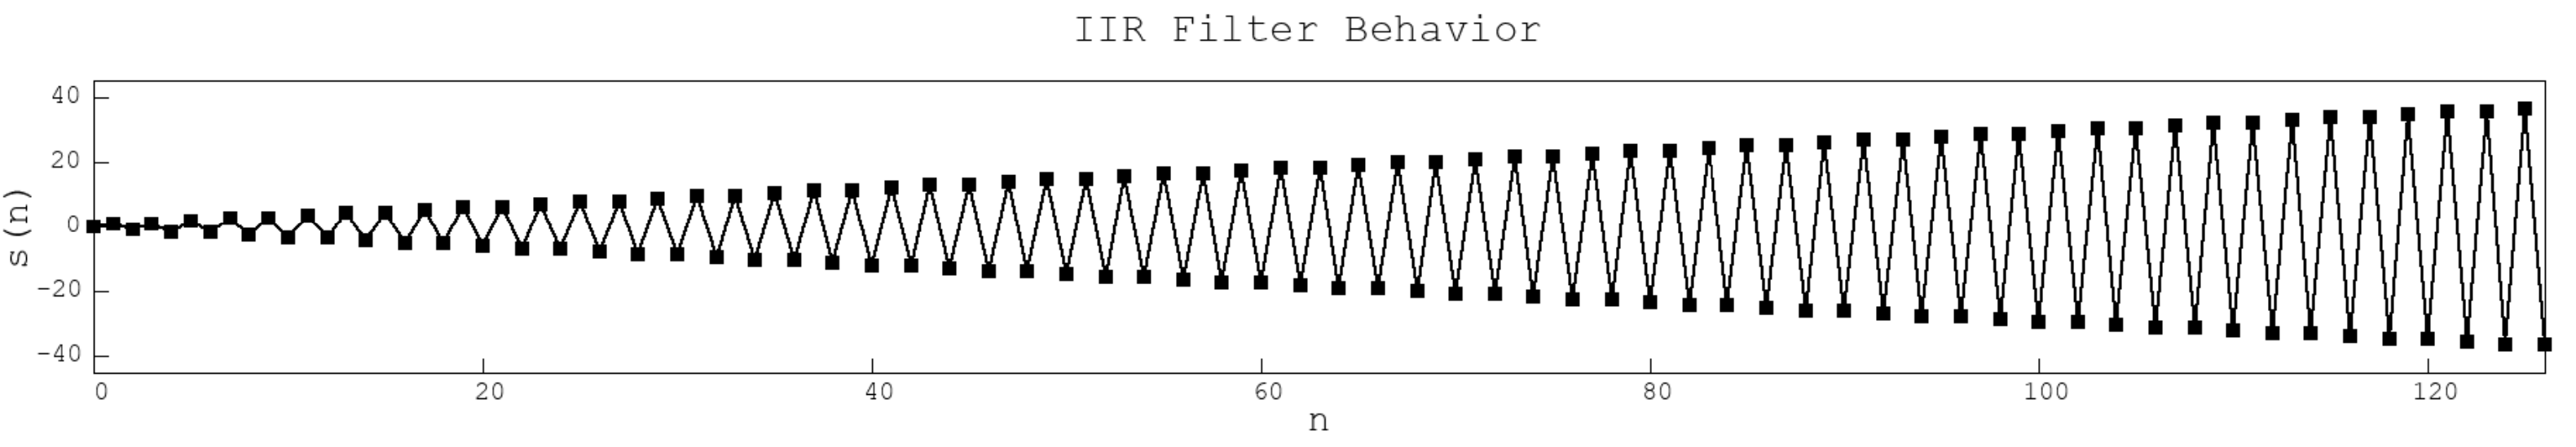
\includegraphics[width=\linewidth]{figs/probe.png}
    \caption{Intermediate signal, $s(n)$, resulting from IIR filter pass of input signal within the \textit{C++} program. (See Ref. \cite{github}).}
    \label{fig:9}
\end{figure*}

Because of the complexity of FPGA designs due to constraints like clocking and fixed-point arithmetic, it can be useful to first simulate a model of the expected mathematical behavior and results of the design in a software language like \textit{Python} or \textit{C++}. Once a model is built (likely one using floating-point arithmetic), the FPGA design can be cross-referenced against the software implementation in order to validate the results and compare accuracy. Of course, the results of software simulations represent an ideal filter in the absence of noise and with generally higher accuracy arithmetic. Simulations can be representative of filter behavior but not necessarily performance.

\bigskip

At this stage, a constraint can be imposed on the system. Assume that the input signal to the Goertzel filter is a purely real signal, i.e. a sine wave. First, populate an array or vector with time values, \verb+t[]+, corresponding to the correct sampling rate. Then, by populating a second array, \verb+x[]+, with the values of $\sin(2\pi f t)$, the desired signal with frequency is obtained in the form of an array of length $N$. (See \textbf{FIG. 7}).
\begin{lstlisting}[language=C++]
    for (i = 0; i < N; i = i + 1)
        x[i] = sin(2PI*f*t[i]);
\end{lstlisting}

Now that a signal has been generated with the desired length and frequency, the Goertzel filter can be implemented. The filter's difference equations must first be rewritten in terms of their explicit real and imaginary parts.
\begin{align}
    s(n) & = x(n) + 2\cos(\varphi)\cdot s(n-1) - s(n-2) \nonumber \\
    \Re{X(k)} & = \cos(\varphi)\cdot s(N-1) - s(N-2) \nonumber \\ 
    \Im{X(k)} & = \sin(\varphi)\cdot s(N-1)
\end{align}
Recall that $x(n)$ is a real-valued sequence, therefore $s(n)$ must also be real-valued because the coefficients of the IIR filter are real. In a \textit{C++} program, complex values must be stored as two real values, and an implementation of the filter might look something like the following:

\begin{lstlisting}[language=C++]
    // IIR Portion of Goertzel Filter
    drs0 = 0;   // s(n)
    drs1 = 0;   // s(n-1)
    drs2 = 0;   // s(n-2)
    SIN = sin(2*pi*k/N);
    COS = cos(2*pi*k/N);
    for (n = 0; n < N; n = n + 1) {
        drs0 = x[n] + 2*COS*drs1 - drs2;
        drs2 = drs1;
        drs1 = drs0;
    }
\end{lstlisting}

Each iteration of the loop, the current output sample, \verb+drs0+, is calculated then proceeded by a shifting of sample values to delay registers (variables stored in memory).

Following the IIR filter pass, the real and imaginary parts of the result, $X(k)$ can be computed. At termination of the loop, $s(N-1)$ is stored in \verb+drs0+ along with $s(N-2)$ in \verb+drs1+.
\begin{lstlisting}[language=C++]
    Xk_re = COS*drs0 - drs1;
    Xk_im = SIN*drs0;
\end{lstlisting}

Of course, the final trivial step remains to calculate the magnitude of $X(k)$. By passing the generated input sequence to this filter for integer $k$-values on the interval $[0, \frac{N}{2}]$, the plot in \textbf{FIG. 8} is obtained. Note that the horizontal axis is shown in units of MHz, as the sampling rate was chosen: $f_s = 100$ MHz. The integer k-values from zero to $\frac{N}{2}$ map to frequency values from zero to the \textit{Nyquist rate}, $f_{N} = f_s/2$. The scaling relation is given by
\begin{equation}
    f = \frac{k}{N} \times f_s
\end{equation}
where $f$ is the "real" frequency measured in Hz. In the example illustrated by \textbf{FIG. 7} and \textbf{FIG. 8}, the signal length was chosen to be $N = 126$ with a sampling frequency of $f_s = 100$ MHz and a signal frequency of $f = 16.67$ MHz. These choices of parameters are not random---for reasons which will be discussed---but in general the choice is arbitrary. As expected, the only non-zero result from the Goertzel filter occurs when $k = 21$, or $f = 16.67$ MHz, where $\abs{X(k)} \approx 63$.

In addition to making predictions of the final results, it is useful to study the internal behavior of the program during the filtering process. \textbf{FIG. 9} shows a plot of the intermediate sequence, \verb+s(n)+, as worked out by the \textit{C++} model. Notably, the sequence oscillates with linearly-increasing amplitude. Obviously, a similar waveform is to be expected within the finalized FPGA design as a form of behavioral validation.

\section{Hardware Implementation}

Now that an expected behavior and result has been defined by the \textit{C++} program, the FPGA device can be programmed and tested.

Commonly, FPGAs are programmed and tested using an \textit{integrated development environment} (IDE) like AMD's \textit{Vivado}. In the form of a \textit{hardware description language} (HDL) like \textit{Verilog} or \textit{VHDL}, code is written to describe the behavior of the internal logic components within the FPGA. The IDE is designed to convert human-readable HDL into a physical circuit (or equivalent schematic) which performs the desired task in a process called \textit{synthesis}. In general, this process is quite different from developing software that might run on a CPU, so there are a couple things one must first understand.

\subsection{HDLs and FPGA Logic}
Writing an algorithm in a hardware description language is considerably different from a standard software language like \textit{Python} or \textit{C++}. HDL is known to be a "lower-level" language in comparison, and as such it can be a bit more difficult to write as requirements become more complex.

\subsubsection{Binary Logic and Fixed-Point Arithmetic}
Hardware components like CPUs and FPGAs operate entirely on the control and manipulation of internal and external signals described by high and low voltages (logic 1s and 0s), thus all variables and operations performed on them require careful consideration of the flow and storage of these \textit{binary} signals. Because of this, all math must be done under the assumption of finite precision, often characterized by the \textit{bit-width} of a particular operation. Because of limited resources within the FPGA, minimizing the number of bits necessary to store a value or perform an operation is an important aspect of optimization.

\textit{Fixed-point arithmetic} is a method of representing fractional values in a binary format by the specification of an "imaginary" decimal point, such that all bits to the right of the decimal point represent fractional values while all bits to the left of the decimal point represent integer values. For example, the decimal value, $(11.625)_d$, can be represented in fixed-point notation as 
\begin{align*}
    (1011.1010)_b & = 2^3 + 2^1 + 2^0 + 2^{-1} + 2^{-3} \\
    & = (11.625)_d
\end{align*}
where four of the 8 bits are assigned as fractional bits. This representation is equivalent to dividing the binary integer value by a \textit{scale factor}, $S = 2^f$, where $f$ is the number of fractional bits. The \textit{accuracy}, $A(f)$, of a  fixed-point binary value is the magnitude of the maximum difference between a real value and its binary representation, defined as half of the resolution, $R(f)$, which is the smallest representable value of the format. (See Ref. \cite{fixed-point}).
\begin{align}
    R(f) & = 2^{-f} \\
    A(f) & = \frac{R(f)}{2} = \frac{1}{2^{f+1}}
\end{align}

It is important to keep in mind that within the FPGA, this decimal point truly is imaginary. All math is generally done in integer binary format (i.e. fixed-point with zero fractional bits assigned) and thus the burden is on the engineer to keep track of the location of the decimal point between operations. As a result, fixed-point arithmetic can quickly add complexity to many FPGA processes.

\textbf{A Note on Notation:} In fixed-point format, unsigned integers are represented as $U(n,f)$, where $n$ is the number of integer bits, and $f$ is the number of fractional bits. The total width (in bits) of an unsigned integer is $n+f$. Signed integers are represented slightly different, as $A(n,f)$, where $n$ and $f$ are the same, but there is an implicit sign bit, such that the total width is $n+f+1$. (See Ref. \cite{fixed-point}).

\subsubsection{Sequential vs. Combinatorial Logic}
As mentioned previously, one of the primary benefits to using an FPGA is the ability to perform many tasks in parallel. Various processes within a chip can run at the same time with their own dedicated logic elements like multipliers and adders. This is often referred to as \textit{combinatorial logic}. This is in contrast with the behavior of something like a CPU which performs most operations sequentially using one or a few \textit{arithmetic and logic units} (ALUs). FPGAs can take advantage of this feature to perform high-complexity operations very quickly in comparison with a processor. 

More intuitively, it can be described via the idea that code is executed one line at a time in a software language, whereas in HDL all code executes simultaneously. While combinatorial logic can be incredibly fast, it is not \textit{instantaneous}. It takes a finite amount of time for a signal to propagate through logical elements. For some intense FPGA processes the \textit{propagation delay} between physical locations within the chip may need to be taken into consideration.

Not all logic within FPGAs can be parallel, however. There are many operations (digital filtering included) which rely on synchronization facilitated by \textit{clocks}.

\subsubsection{Clocking}

\textit{Clocks} are one of the most important logical elements of FPGAs and other processing systems. They act as the primary driver of activity within the system, and are used for performing sequential (time-dependent) operations. Simply put, a clock is a special internal signal which switches between logical zero and one (low and high voltage) at a particular \textit{clock frequency}. This behavior is usually driven by an independent hardware component such as a crystal oscillator.

Often times, sequential FPGA logic is characterized by the behavior of the system at each \textit{rising edge} of the clock. Essentially, each low-to-high transition of the clock drives other signals to change and propagate through the logic gates. As a result, a higher clock frequency is generally synonymous with faster calculations. For example, the \verb+always+ statement is commonly used to instantiate sequential logic in Verilog:
\begin{lstlisting}[language=Verilog]
    always @ (posedge clk) begin
        if (rst) n <= 0;
        else n <= n + 1;
    end
\end{lstlisting}

The above code effectively acts as a sequential counter driven by the clock. Each positive edge of \verb+clk+, the code within the \verb+always+ block (bounded by \verb+begin+ and \verb+end+) is executed exactly once, in parallel. It is common to use signals like \verb+rst+ (reset) to conditionally facilitate behavior of logical elements like this counter.

\begin{figure}
    \centering
    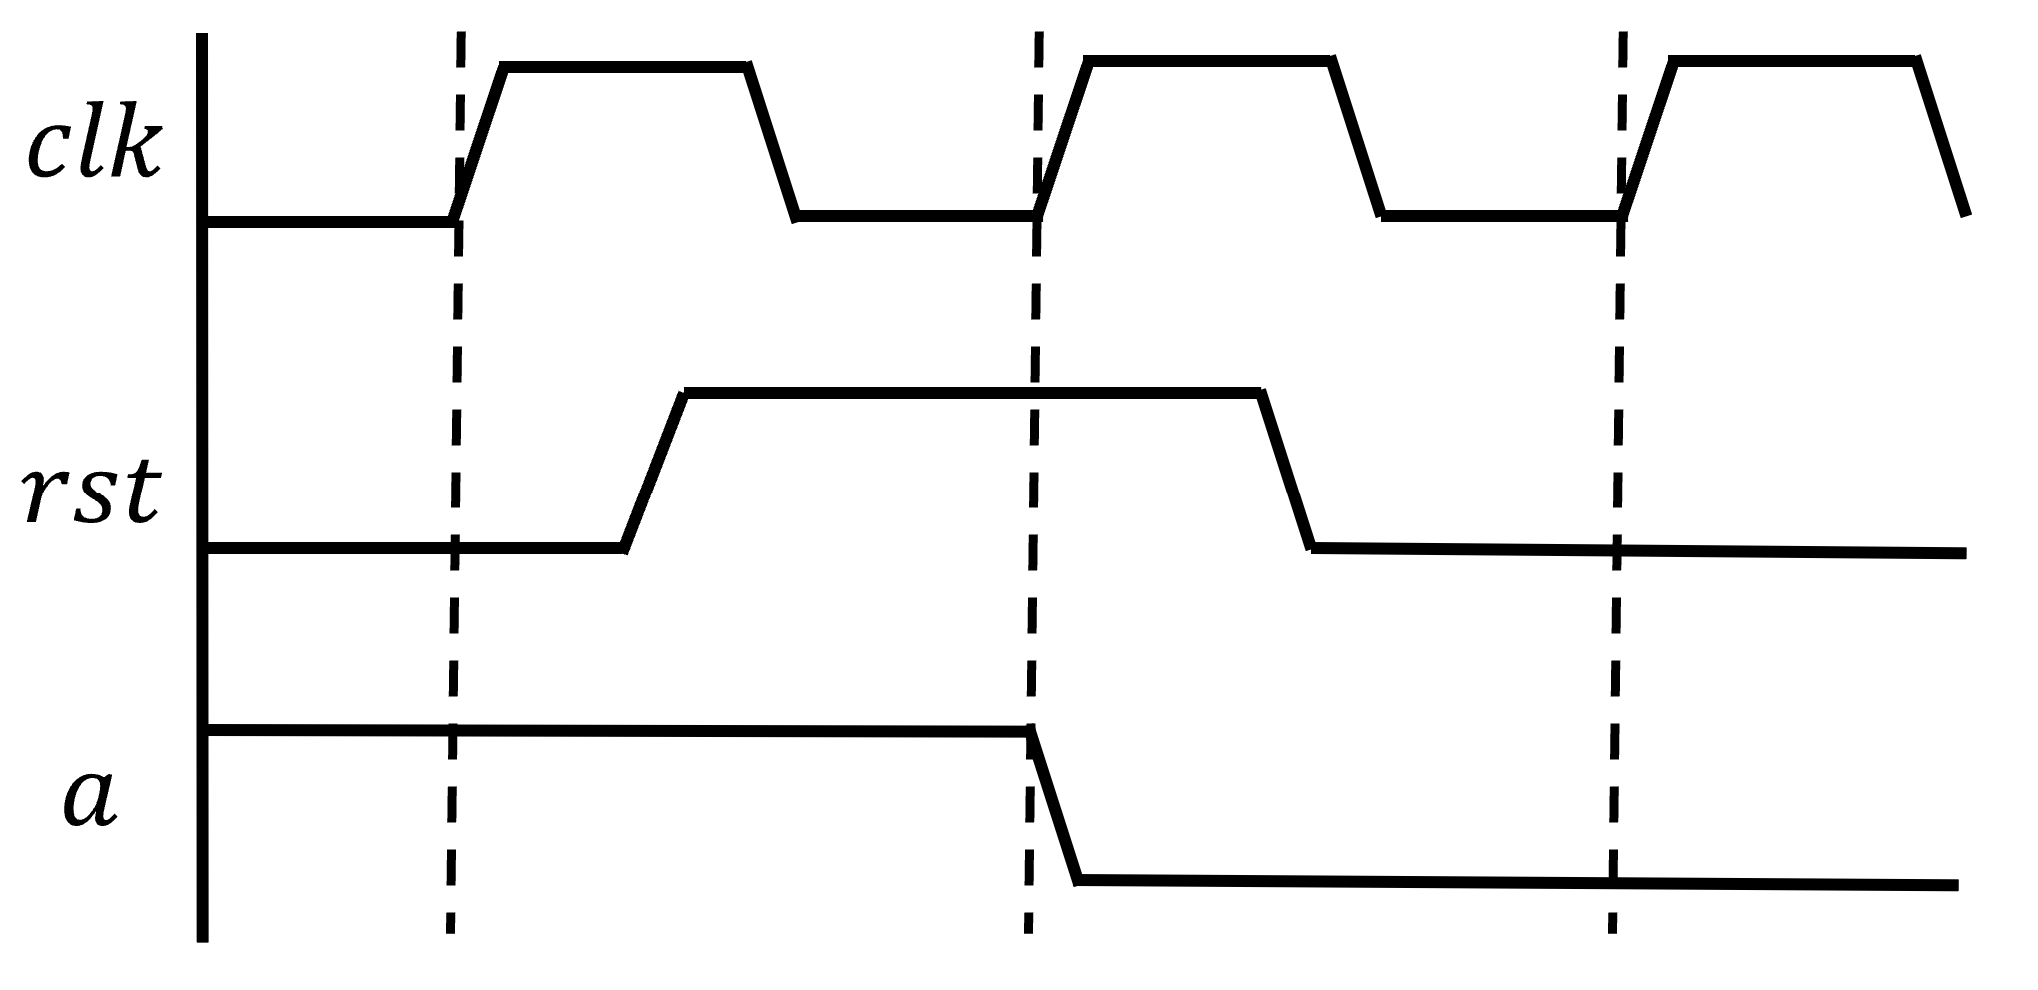
\includegraphics[width=\linewidth]{figs/logic_signals.png}
    \caption{Waveform diagram of sequential FPGA logic. The vertical dashed lines are used to emphasize the location of rising edges of the clock. While the $rst$ signal is high for some time, the target signal, $a$, remains unaffected until the next rising $clk$ edge occurs.}
    \label{fig:10}
\end{figure}

Waveform diagrams like the one in \textbf{FIG. 10} are often used to analyze and debug the behavior of a particular segment of HDL. Variables or signals within the hardware are represented as a waveform with time on the horizontal axis. The vertical axis of each signal represents its value, either zero or one (low or high) for signals like a clock or reset, or a full binary integer representation for signals that are more than a single bit wide. 

\textbf{FIG. 10} provides an example of how sequential behavior might look in an FPGA design. Imagine \textit{Verilog} code such that at each rising edge of the clock, the value \verb+a+ is reset to logic zero if the \verb+rst+ signal is high. Evidently, the \verb+rst+ signal is active for some time before the next rising edge of the clock finally drives \verb+a+ to zero. The code to describe this behavior is as follows.
\begin{lstlisting}[language=Verilog]
    always @ (posedge clk) begin
        if (rst) a <= 0;
    end
\end{lstlisting}

Understanding \textit{clocking} is one of the first steps to programming FPGAs.

\subsection{Further Simplification of the Filter}

As one final touch on formalism before writing and testing \textit{Verilog} code for an implementation of this filter, it can be simplified even further to eliminate the need for a few multiplications. The IIR component has the transfer function
\begin{equation}
    H_{IIR}(z) = \frac{1}{1-2\cos(2\pi k/N)z^{-1} + z^{-2}}
\end{equation}

Recall that the choice of window size, $N$, is generally arbitrary. The primary goal of using this filter is to detect a consistent Fourier coefficient for a single frequency between zero and Nyquist in order to validate the output of an ADC, thus any input frequency will produce predictable results. Evidently, then, the integer $k$-value is also arbitrary, and can be chosen such that the $2\cos(2\pi k/N)$ coefficient in the transfer function is eliminated entirely.

In the \textit{C++} testbench, a window size of $N = 126$ was chosen, as well as an input signal frequency of $f = \frac{f_N}{6} = 16.67$ MHz. While these values are seemingly random, they were chosen intentionally such that the non-zero value from the Goertzel filter would be expected at $k = \frac{N}{6} = 21$. With $k = 21$ and $N = 126$ set in place as constants, \textit{Niven's theorem} can be applied. This theorem (see Ref. \cite{niven}) states that the only values of $\varphi \in [0,\pi/2]$ for which $\varphi/\pi$ and  $\sin(\varphi)$ are both rational numbers are:
\begin{align}
    \sin(0) & = \cos(\frac{\pi}{2}) = 0 \nonumber \\
    \sin(\frac{\pi}{6}) & = \cos(\frac{\pi}{3}) = \frac{1}{2} \\
    \sin(\frac{\pi}{2}) & = \cos(0) = 1 \nonumber
\end{align}
Exploiting this fact, $k$ and $N$ can be chosen such that
\begin{align}
    \frac{k}{N} & = \frac{1}{6}  \implies \varphi = \frac{2\pi k}{N} = \frac{\pi}{3} \nonumber \\ 
    & \therefore 2\cos(\frac{2\pi k}{N}) = 1
\end{align}
which eliminates the only multiply remaining in the IIR filter. The new transfer function is given by
\begin{equation}
    H_{IIR}(z) = \frac{1}{1 - z^{-1} + z^{-2}}
\end{equation}
with the resulting difference equation
\begin{equation}
    s(n) = x(n) + s(n-1) - s(n-2)
\end{equation}

See \textbf{FIG. 11} for a plot of the resulting transfer function, which has one zero and two poles as expected.

\begin{figure}
    \centering
    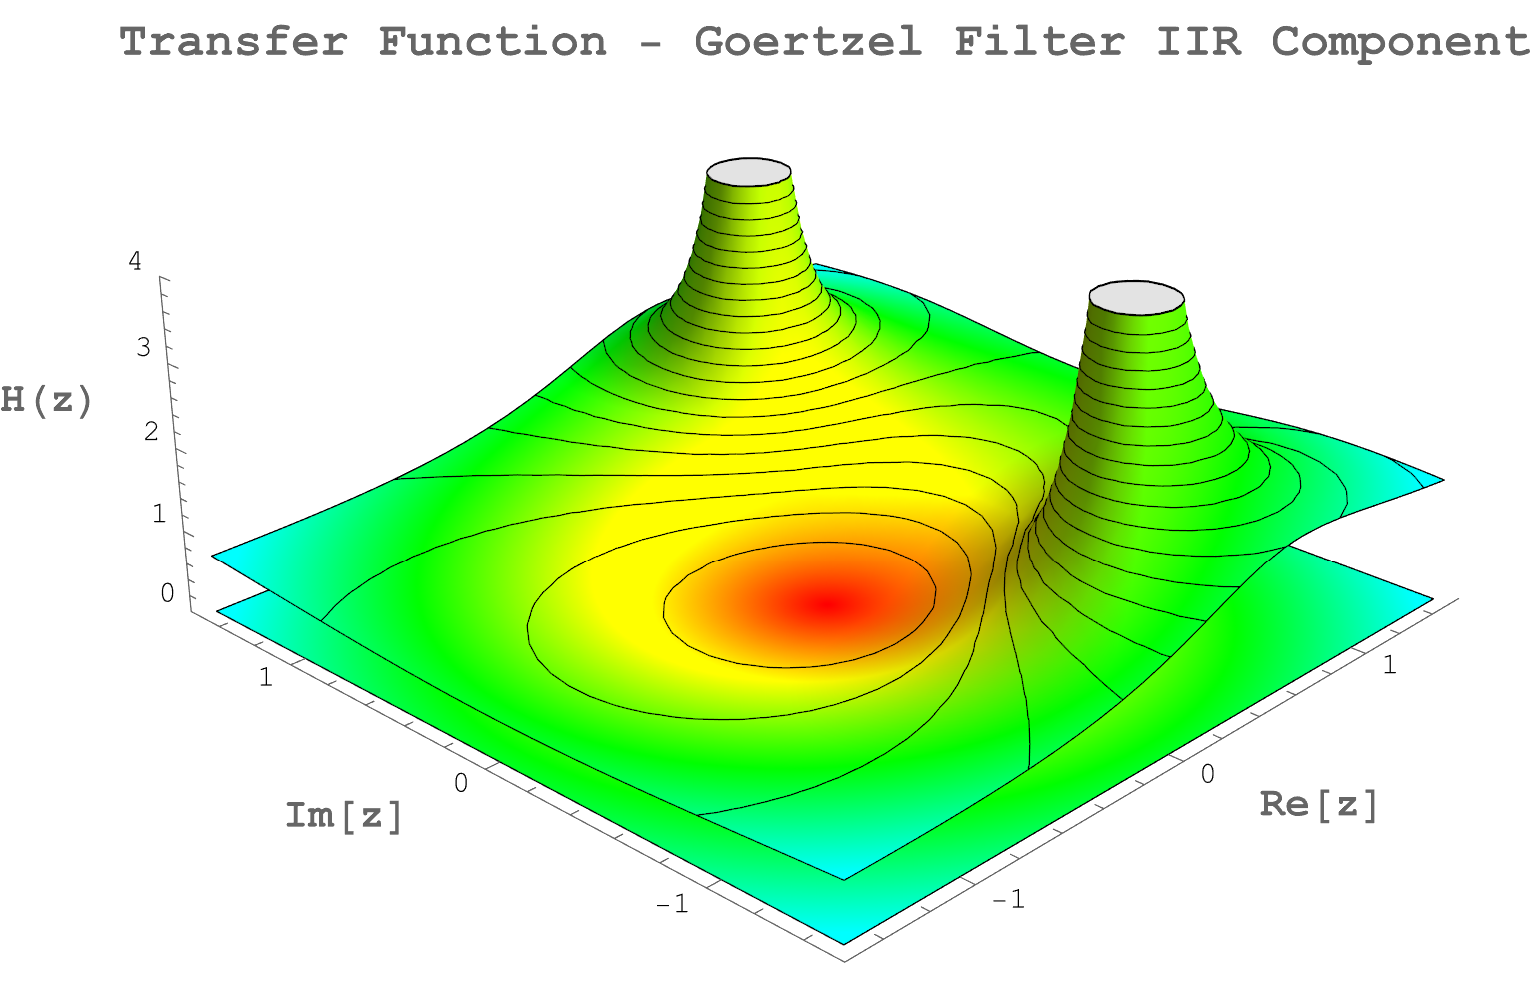
\includegraphics[width=\linewidth]{figs/transfer_function.png}
    \caption{Transfer function for the IIR component of the simplified Goertzel filter. As expected, the function has a zero at the origin. It also has two poles, each on the unit circle. Thus, the filter is \textit{marginally stable}. See equation \textbf{(30)}. }
    \label{fig:11}
\end{figure}

Relatively speaking, the final form has an incredibly small resource requirement. Digital filters may often require over one hundred taps (coefficients)! The Goertzel filter's IIR portion can be implemented with only two adders and two delay registers for storage of the previous two output values, $s(n-1)$ and $s(n-2)$. The FIR portion immediately follows (in simplified form) from equation \textbf{(23)}.

\begin{align}
    \Re{X(k)} & = \frac{1}{2} s(N-1) - s(N-2) \nonumber \\ 
    \Im{X(k)} & = \frac{\sqrt{3}}{2} s(N-1)
\end{align}

\subsection{The RFSoC}

A \textit{system-on-chip} (SoC) is generally defined as any single electronic chip which contains all of the components necessary for a complete, functioning electronic system. In the FPGA industry, a SoC usually integrates the traditional programmable logic (PL) of an FPGA alongside a \textit{processing system} (PS), internal memory blocks, and input/output ports on a single chip.

\textit{AMD's} RFSoCs (\textit{radio-frequency systems-on-chip}) are a series of the most powerful and fastest clocked FPGAs that the current state of the art produces. Radio-frequency experiments like CoRaLs and PUEO utilize these FPGAs---integrated with custom hardware---to achieve the highest possible efficiencies of data processing, filtering, and triggering as required by the experiments. 

The ADCs on the RFSoC produce 12-bit (signed integer) samples at 3 GSPS (giga-samples per second), providing an observational bandwidth up to 1500 MHz. The system clock runs at 375 MHz, which effectively translates to 375 million operations per second \textit{for each independent parallel process}. Since the ADCs sample at eight times the rate of the system clock, we expect to obtain exactly eight signal samples per clock cycle.

Remember, many signals only propagate through the logic elements on every rising edge of the clock. As a result, processing multiple samples per clock cycle is especially difficult for an IIR filter, since values of the output sequence depend on values within the same clock cycle that haven't been calculated yet. With FIR filters, the process can be managed with \textit{pipelining}.

If the Goertzel implementation takes one out of every eight samples, or perhaps one out of every sixteen samples (one of eight every other clock cycle), then it doesn't much matter that the ADCs sample faster than the system clock, because the Goertzel filter only receives data at one sample per clock cycle (or two), and the implementation is as straightforward as any. This introduces a much lower Nyquist frequency---since the Goertzel filter effectively "samples" at 1/8 or 1/16 of the ADC rate---above which aliasing occurs.

\subsection{Choosing Parameters}

Remember, the end goal is to detect the presence and consistency of a controlled, continuous-wave, external signal which is converted by the ADCs. Frequency of this signal must be chosen so that 
\begin{enumerate}
    \item The signal is out of the target frequency band for observations so as not to interfere with experimental data.
    \item The signal is below the effective Nyquist rate of the Goertzel filter.
    \item The signal can be detected at an integer $k$ value such that $k/N = 1/6$. 
\end{enumerate}

Recall the scaling relation between $k$ and a real signal frequency, measured in Hz as given by equation \textbf{(24)}. The requirement $k/N = 1/6$ means that the controlled signal frequency must be one-sixth of the sampling rate. Thus, the second condition is automatically satisfied by the third since the \textit{Nyquist rate} is defined as exactly half of the sampling rate.

Given the RFSoC's ADC sampling rate of 3 GSPS, decimating the signal by a factor of eight or sixteen corresponds to a Goertzel filter sample rate of 375 MSPS or 187.5 MSPS, respectively. Equation \textbf{(24)} then yields possible controlled signal frequencies.

\begin{align}
    f_i & = 62.5 \text{ MHz @ } f_s = 375 \text{ MSPS} \nonumber \\
    f_i & = 31.25 \text{ MHz @ } f_s = 187.5 \text{ MSPS} \nonumber
\end{align}

For the sake of satisfying the first requirement, the lower frequency is preferred, thus the Goertzel filter takes one of every 16 ADC samples in implementation.

The number of samples collected for the filtering process of the Goertzel algorithm, $N$, is generally arbitrary. In practice, however, there are three constraints. 
\begin{enumerate}
    \item The \textit{rate of conversion} is inversely proportional to number of samples, $N$.
    \item The \textit{resource requirement} (bit width) of the IIR component is logarithmically proportional to $N$.
    \item N must be a multiple of six such that $k/N = 1/6$ yields an integer $k$
\end{enumerate}

\subsubsection{Rate of Conversion}

As highlighted previously, the value $X(k)$ produced by the Goertzel algorithm---which will be referred to as the \textit{Goertzel coefficient}---requires the accumulation of $N$ samples to obtain the final values of the intermediate sequence, $s(N-1)$ and $s(N-2)$ (See equation \textbf{(23)}). Only after all N samples are obtained can the Goertzel coefficient be calculated, so the rate at which the filter produces a new valid coefficient (the \textit{rate of conversion}) is limited to

\begin{equation}
    \text{ROC} \leq  \frac{f_s}{N} 
\end{equation}
where $f_s$ is the \textit{decimated} sample rate of the Goertzel filter rather than the full 3 GSPS of the RFSoC's ADCs. Evidently, the chosen value of the parameter $N$ is dependent on how often the consistency of the continuous wave is to be verified.

\begin{figure}
    \centering
    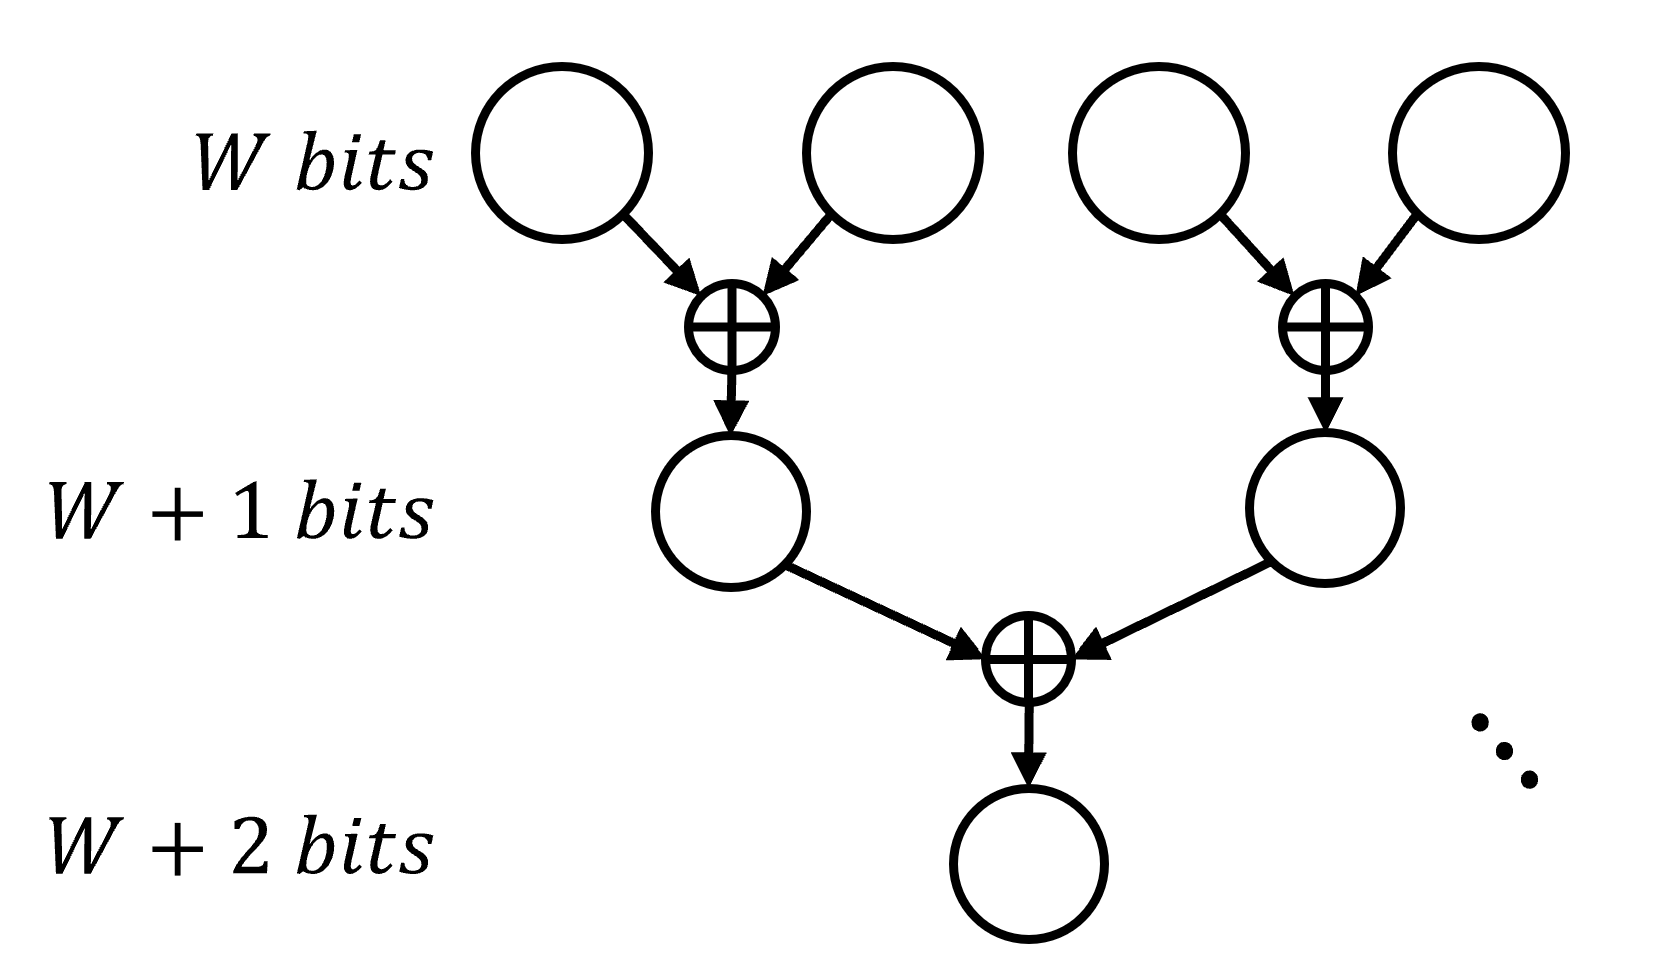
\includegraphics[width=\linewidth]{figs/binary_addition_tree.png}
    \caption{Binary addition tree: a useful representation of bit growth based on number of additions. For N terms added, the necessary width is $W + \lceil\log_2(N)\rceil$.}
    \label{fig:12}
\end{figure}

\subsubsection{IIR Component Resource Requirement}

In binary arithmetic, the bit width needed to store the sum of two values of width $W$ is $W+1$ (See Ref. \cite{fixed-point}). Adding together four values of width $W$ yields two values of width $W+1$, which each add together for a final width of $W+2$. For accumulation of eight values of width $W$, obviously $W+3$ bits are needed, and so on. Evidently, adding together $N$ values of width $W$ requires a final width of $W + \lceil\log_2(N)\rceil$. In the implementation of the IIR component of the filter (see equation \textbf{(31)}), there are two additions per sample. The initial width corresponds to the width of the signal, which is 12-bit data coming directly from the ADCs. It follows from the above reasoning that the number of bits required to store the values of the intermediate sequence is
\begin{equation}
    Q = 12 + \lceil\log_2(2N)\rceil
\end{equation}

With these proportionalities in mind, $N = 128$ makes for a reasonable choice of window size. This requires eight additional bits for the intermediate sequence on top of the 12-bit signal width, resulting in $s(n)$ values stored at 20 bits. However, the third constraint on $N$ imposes the requirement that $N$ is a multiple of 6. The nearest candidate is $N = 126$, meaning that a signal of $f_i = 31.25$ MHz will map to an integer-valued $k = 21$ as demonstrated in the software implementation. The resulting ROC is $\sim 1.5$ MHz, obtained by plugging in values to equation \textbf{(33)}.

To summarize the chosen parameters, bit widths, and properties of both the RFSoC and the filter:

\begin{align}
    f_{s} & = 3 \text{ GSPS \ \ \ \ \ \ \ (ADC)} \nonumber \\
    f_{s} & = 187.5 \text{ MSPS \ (Filter)} \nonumber \\
    f_{i} & = 31.25 \text{ MHz} \nonumber \\
    W_{x(n)} & = 12b \nonumber \\
    Q_{s(n)} & = 20b \nonumber \\
    N & = 126 \nonumber \\
    k & = 21 \nonumber \\
    |X(k)| & = 63 \nonumber
\end{align}

\subsection{The Implementation}

\begin{figure*}
    \centering
    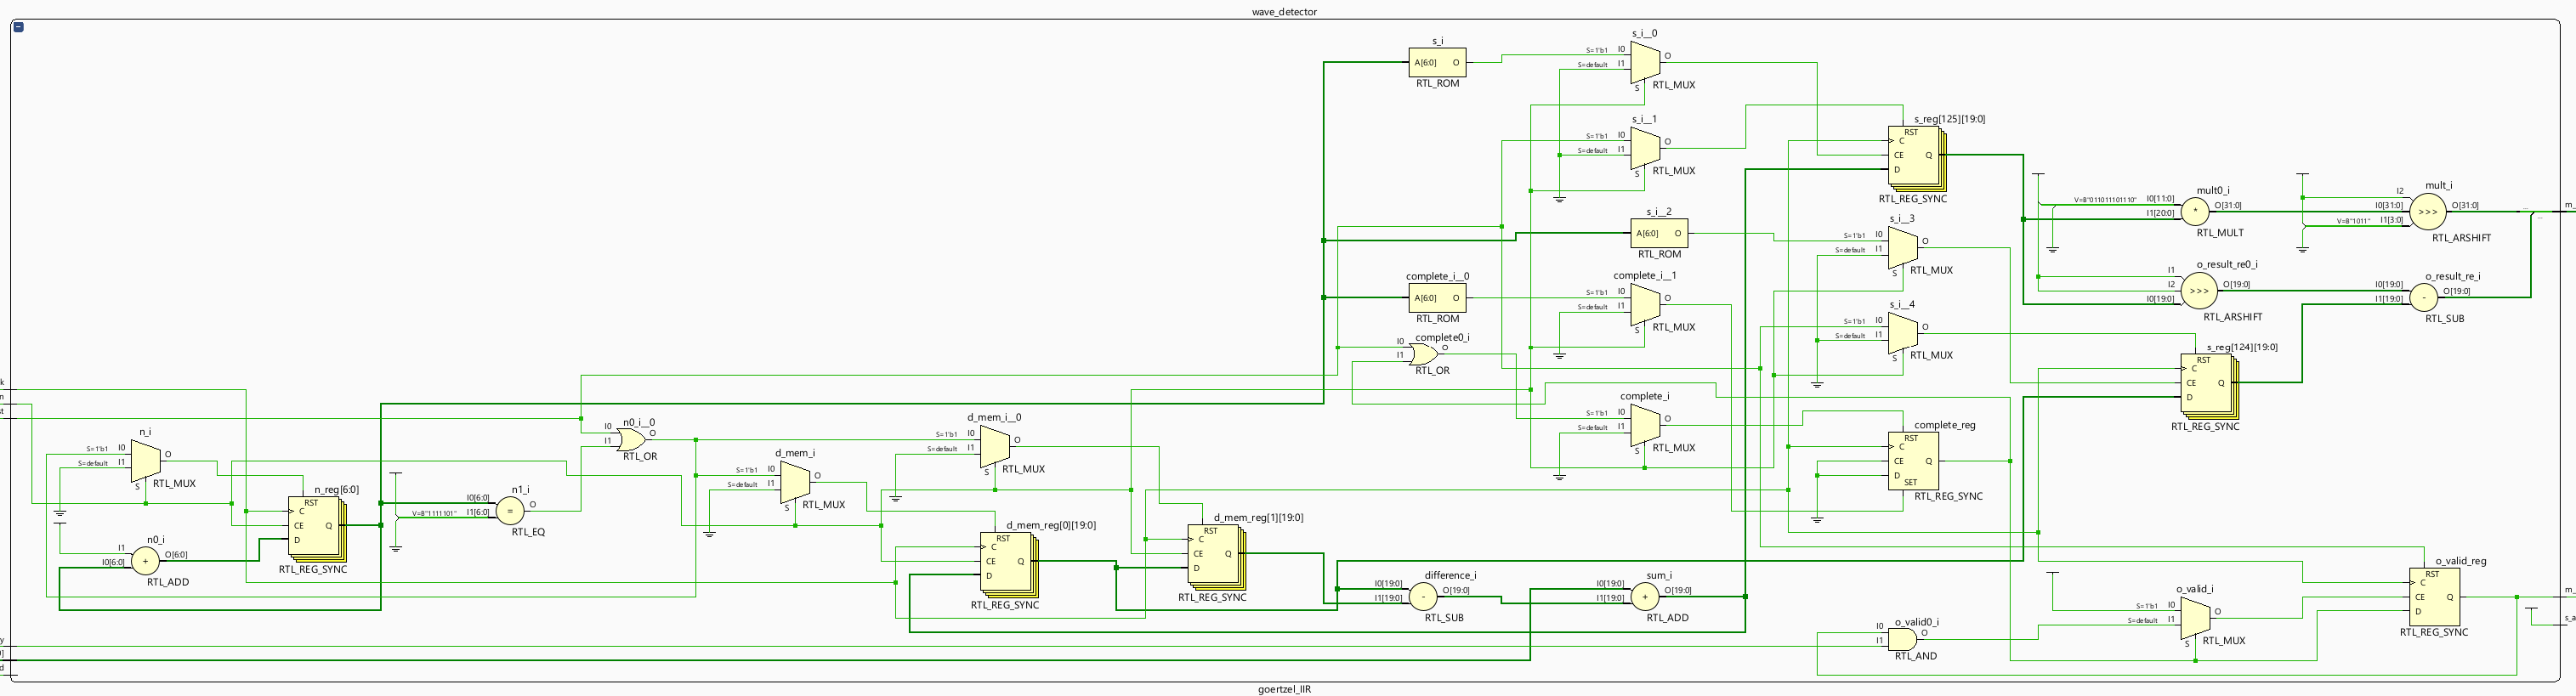
\includegraphics[width=\linewidth]{figs/bd_goertzel.png}
    \caption{\textit{\textbf{Vivado}} generated block diagram of the final HDL implementation of the Goertzel filter design. The design appears rather complex because Vivado does not care much about visual organization, but the module can be treated as a "black box" such that the user does not care what is going on inside.}
    \label{fig:13}
\end{figure*}

\begin{figure}
    \centering
    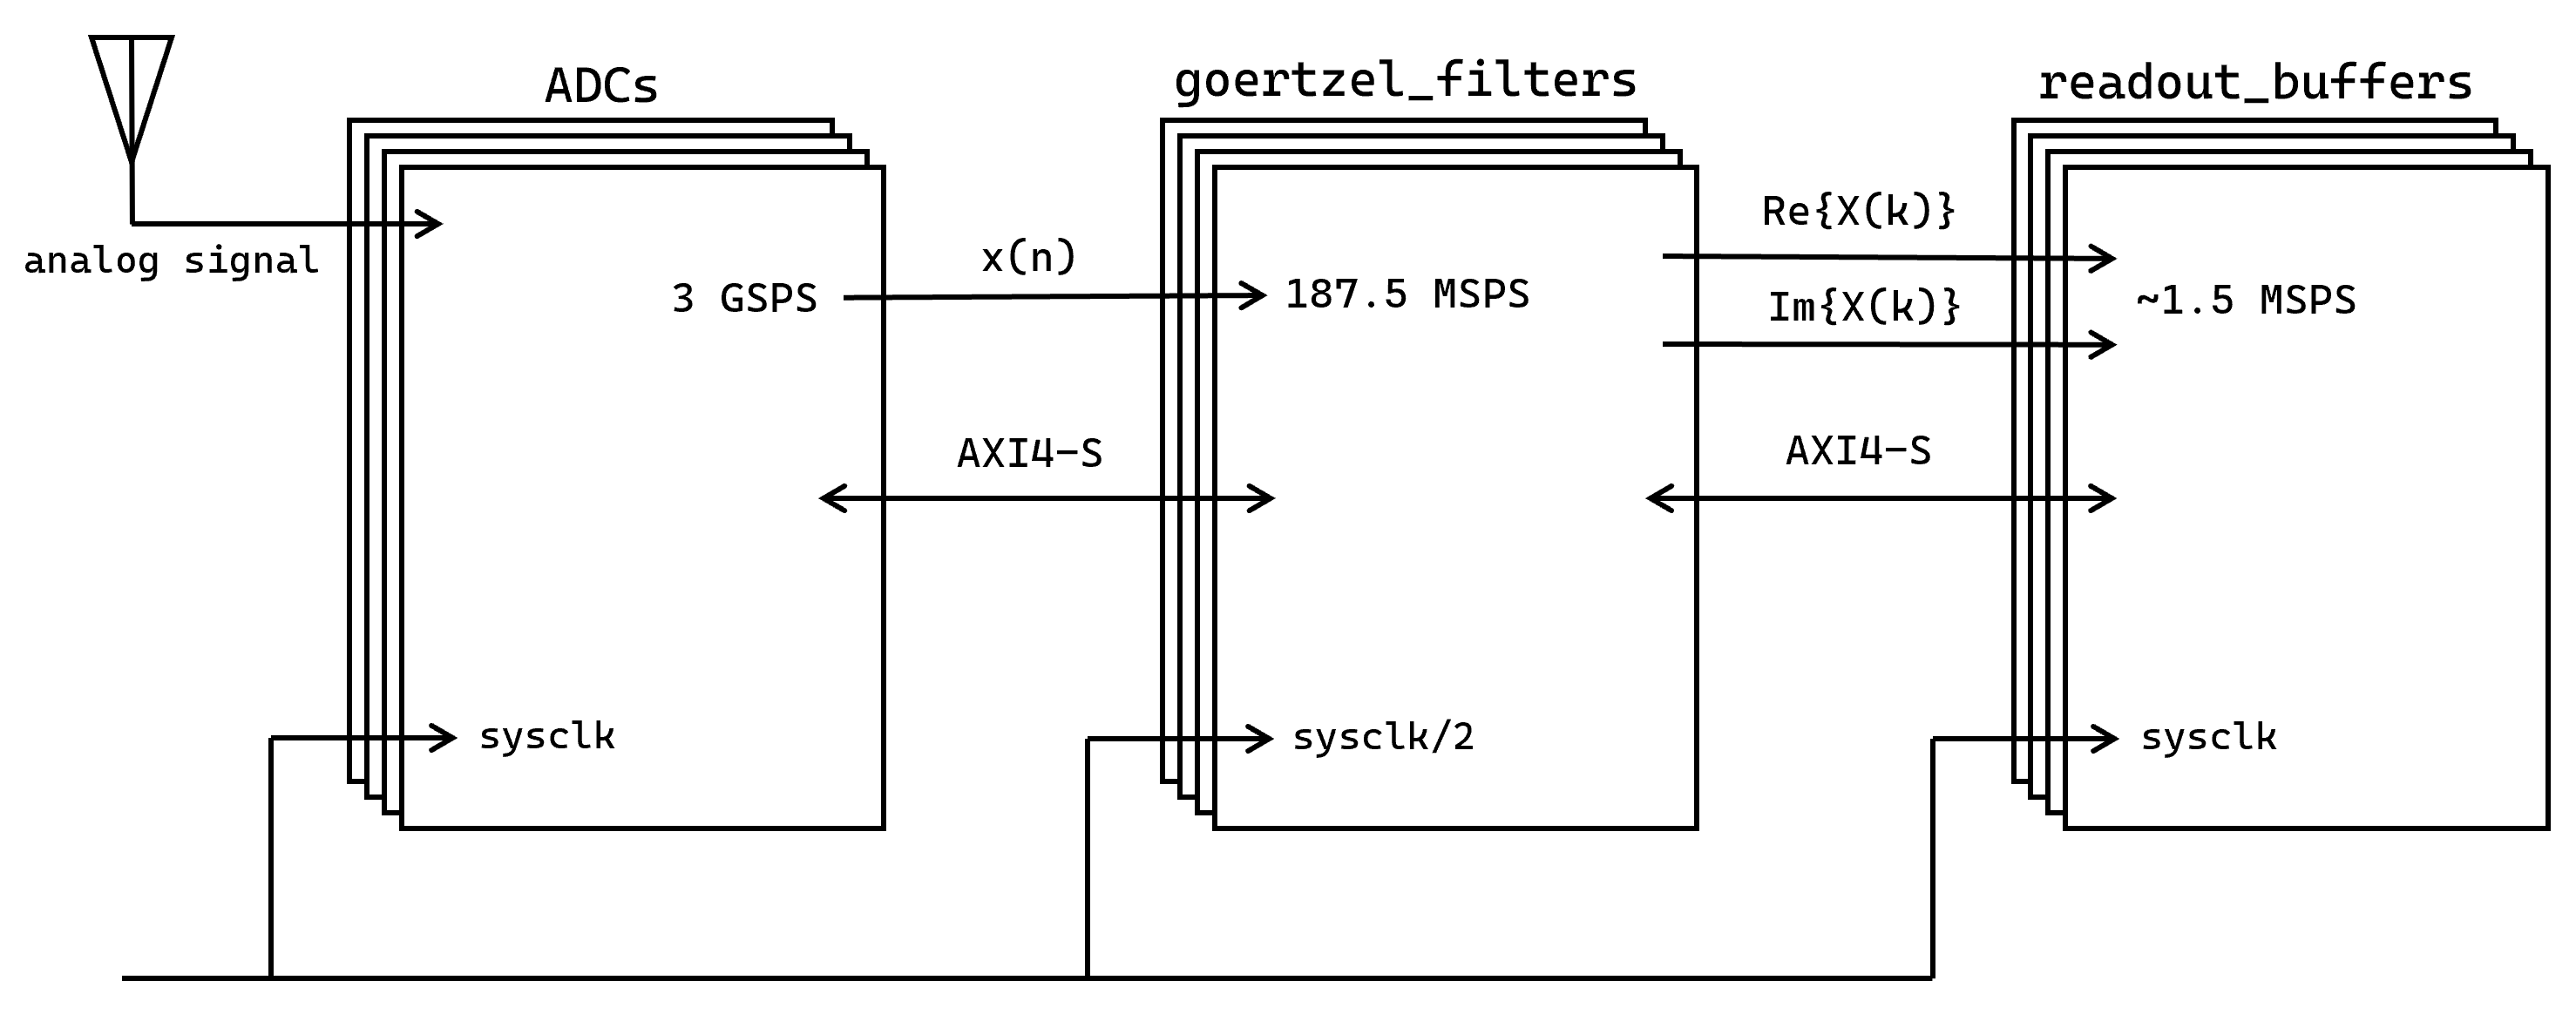
\includegraphics[width=\linewidth]{figs/bd_goertzel_simple.png}
    \caption{Simplified block diagram illustrating the integration of the Goertzel filter with firmware elements like the ADCs and readout buffers for testing.}
    \label{fig:14}
\end{figure}

The final HDL implementation of the filter is composed of two main stages---the IIR and FIR portions are separated in the cascade form. The IIR filter component is a synchronous process which relies on $N = 126$ samples correctly counted and accumulated according to the difference equation \textbf{(31)}. Once 126 samples are received and intermediate samples $s(N-1)$ and $s(N-2)$ are obtained, the FIR portion of the filter (or rather, the algebraic simplification of it, equation \textbf{(32)}) can proceed and send valid data to the filter's output registers. A block-diagram of the filter as is generated by Vivado looks like a bit of a mess (see \textbf{FIG. 13}), but it can be simplified by considering the sub-components of the design separately.

\subsubsection{Counting Samples}
The filter must keep track of the number of samples which have been accumulated. Verilog code for this is straightforward.

\begin{lstlisting}[language=Verilog]
    reg [7:0] n = 0;
    always @ (posedge i_clk) begin
        if (i_clken) begin
            if ( i_rst || n == (N-1) ) n <= 0;
            else n <= n + 1;
        end
    end
\end{lstlisting}

The counter only operates while \verb|i_clken| is high, and the value of \verb|n| returns to zero on two conditions. Either on assertion of a synchronous reset signal, \verb|i_rst|, or when $N$ samples have been seen. Each "falling edge" of this signal tells the rest of the design when the IIR filtering process has completed.

\subsubsection{Delay Registers}

As the IIR filter operates, it needs two signed 20-bit registers to store past values of the sequence, \verb|d_mem[0]| and \verb|d_mem[1]|. Both registers must be initialized to zero.
\begin{lstlisting}[language=Verilog]
    reg signed [19:0] d_mem [1:0];
    initial begin
        d_mem[0] = 0;
        d_mem[1] = 0;
    end
\end{lstlisting}

Each clock cycle, the first delay register gets the value of the most recent value of $s(n)$, while the second delay register gets the most recent value of the first delay register. This structure is often referred to as a \textit{shift register}, as the signal can be thought of as "shifting" down the line of delay registers on each clock cycle. The process is implemented like so:
\begin{lstlisting}[language=Verilog]
    always @ (posedge i_clk) begin
        if (i_clken) begin
            if ( i_rst || (n == (N-1)) ) begin
                d_mem[0] <= 0;
                d_mem[1] <= 0;
            end else begin
                d_mem[0] <= sum;
                d_mem[1] <= d_mem[0];
            end
        end
    end
\end{lstlisting}

 Once again the behavior is controlled by the clock enable signal, \verb|i_clken|, and the delay registers reset to zero---either when the filter is reset externally with \verb|i_rst| or when a conversion is finished after 126 samples have been seen. 

\subsubsection{IIR Difference Equation}
 
 The value \verb|sum| in the previous code block is the 20-bit result of fairly simple combinatorial logic used to implement the IIR difference equation \textbf{(31)}:

\begin{lstlisting}[language=Verilog]
    wire [19:0] diff = d_mem[0] - d_mem[1];
    wire [19:0] sum = i_signal + diff;
\end{lstlisting}
where \verb|i_signal| is the 12-bit input signal, $x(n)$. Recall that combinatorial logic does not rely on the clock. Rather, the result is calculated as fast as the electrical signals can propagate through the logical multipliers, adders, or whatever else is present. The fact that \verb|wires| are used for this as opposed to clocked \verb|registers| serves as an explicit reminder of the combinatorial nature. Effectively, the current value of the signal, $s(n)$ or \verb|sum|, is calculated near instantaneously after the current sample, $x(n)$ or \verb|i_signal|, is obtained at each rising clock edge. At the next clock edge, \verb|sum| is simultaneously sent to the first delay register, $s(n-1)$ or \verb|d_mem[0]|, as a new sample arrives.

\subsubsection{FIR Pre-Logic}

Remember, only after 126 samples are seen can the filter obtain the values needed for the FIR component, $s(N-1)$ and $s(N-2)$. Thus, on the clock cycle that $n = N-1$, the filter must capture the current value of \verb|sum| and \verb|d_mem[0]| since
\begin{align}
    \left. s(n) \right|_{n=N-1} = s(N-1) \nonumber \\
    \left. s(n-1) \right|_{n=N-1} = s(N-2)
\end{align}

In HDL, this looks quite lengthy. Once again, registers must be initialized to zero, return to zero on reset, and otherwise their values must only change once per conversion on the correct clock cycle.

\begin{lstlisting}[language=Verilog]
    reg signed [19:0] s [(N-1):(N-2)];
    initial begin
        s[N-1] = 0;
        s[N-2] = 0;
    end
    always @ (posedge i_clk) begin
        if (i_clken) begin
            if ( i_rst ) begin
                    s[N-1] <= 0;
                    s[N-2] <= 0;
            end else if ( n == (N-1) ) begin
                    s[N-1] <= sum;
                    s[N-2] <= d_mem[0];
            end
        end
    end
\end{lstlisting}

Once these values are obtained (every 126 clock cycles), the remaining portion of the filter follows as a simple translation of equation \textbf{(32)} into synthesizable Verilog. 

\subsubsection{FIR Difference Equation}

\begin{lstlisting}[language=Verilog]
    integer [11:0] SIN = 12'd1774;
    wire [31:0] mult = (SIN * s[N-1]) >>> 11;

    wire [19:0] Xk_re = (s[N-1]>>>1) - s[N-2];
    wire [19:0] Xk_im = mult[19:0];  
\end{lstlisting}

This code may be hard to decipher for someone unfamiliar with HDL, thus it needs quite a bit of explanation. It suffers in part from the fact that floating-point operations like multiplying by $\sin(\pi / 3) = \frac{\sqrt{3}}{2}$ are simply impossible in most FPGA applications. The multiplication must be "approximated" by instead multiplying by an integer representation of the sine factor followed with an arithmetic bit shift to the right (\verb|>>>|). In fixed-point arithmetic, a bit shift by $q$ bits is equivalent to a division by a factor $2^q$ (See Ref. \cite{fixed-point}). For example,
\begin{align*}
    010000_b >>> 3 = 000010_b
\end{align*}

The above binary operation is equivalent to the following decimal operation:
\begin{align*}
    16 / 2^{3} = 2
\end{align*}

It's a quite simple example, but it illustrates the point. In decimal, floating-point form, $\sin(\pi/3) \approx 0.8660254...$ To approximate this with an integer multiplication followed by a bit shift, reverse the process beginning with the floating-point form.
\begin{align*}
    \sin(\pi/3) \cdot 2^{11} \approx 1773.62002...
\end{align*}

Rounded to the nearest integer, this gives us an approximation to $\sin(\pi / 3) = \frac{\sqrt{3}}{2}$.
\begin{align}
    1774 / 2^{11} = 0.8662109375
\end{align}
thus the multiplication needed to implement the factor of $\frac{\sqrt{3}}{2}$ is instead a multiplication by 1774 and a bit shift by 11.

Since the integer was rounded up, this yields an overestimate by $\sim 0.0002$. If greater accuracy is needed, the process of choosing a larger bit shift (and thus a larger bit width for the multiplication) is straightforward. 

In the implementation, the signal values $x(n)$ and $s(n)$ may be negative, so they are internally represented as signed \textit{two's complement} integers and must be treated as such in multiplication operations. For brevity, this detail is left out of the code snippets, but is the reason why storing \verb|SIN| = 1774 requires 12 bits as opposed to 11. The product of two signed binary values of width $n$ and $m$ requires a width of $n+m$ (see Ref. \cite{fixed-point}), thus the product of \verb|SIN| (12-bit) and \verb|s[N-1]| (20-bit) must be an intermediate 32-bit value. Since the multiplication by $\sim 0.866$ should result in a \textit{smaller} value than the original 20-bit integer, the intermediate value \verb|mult| can be truncated to just the bottom 20 bits to obtain $Re\{X(k)\}$. 

The imaginary component is much more self-explanatory, with a single bit shift to the right for the factor of $1/2$.

\subsubsection{Support Logic and Interfaces}

At this point in time, the most important logic within the implementation shown by the block diagram (\textbf{FIG. 13}) has been isolated. The remaining clutter is attributed mostly to support logic necessary for the module to interact with the rest of the system it is a part of. These logical elements generally include control flags and the \textit{\textbf{AXI4-Stream Interface}}. For the most part, this logic is use-case specific.

In general, the \textit{AXI4-Stream Interface} acts as the communication channel between modules. Control flags within each module tell neighboring modules when data is ready to be read or written across the available channels in such a manner that prevents data loss or corruption. For example, a filter must communicate to the memory buffers when its data is valid, and the memory buffers must "agree" to receive the data. As such, the \textit{AXI4-Stream interface} is simply a handshake between firmware components along the chain of data processing. See the appendix for details. 

\begin{figure*}[t!]
    \centering
    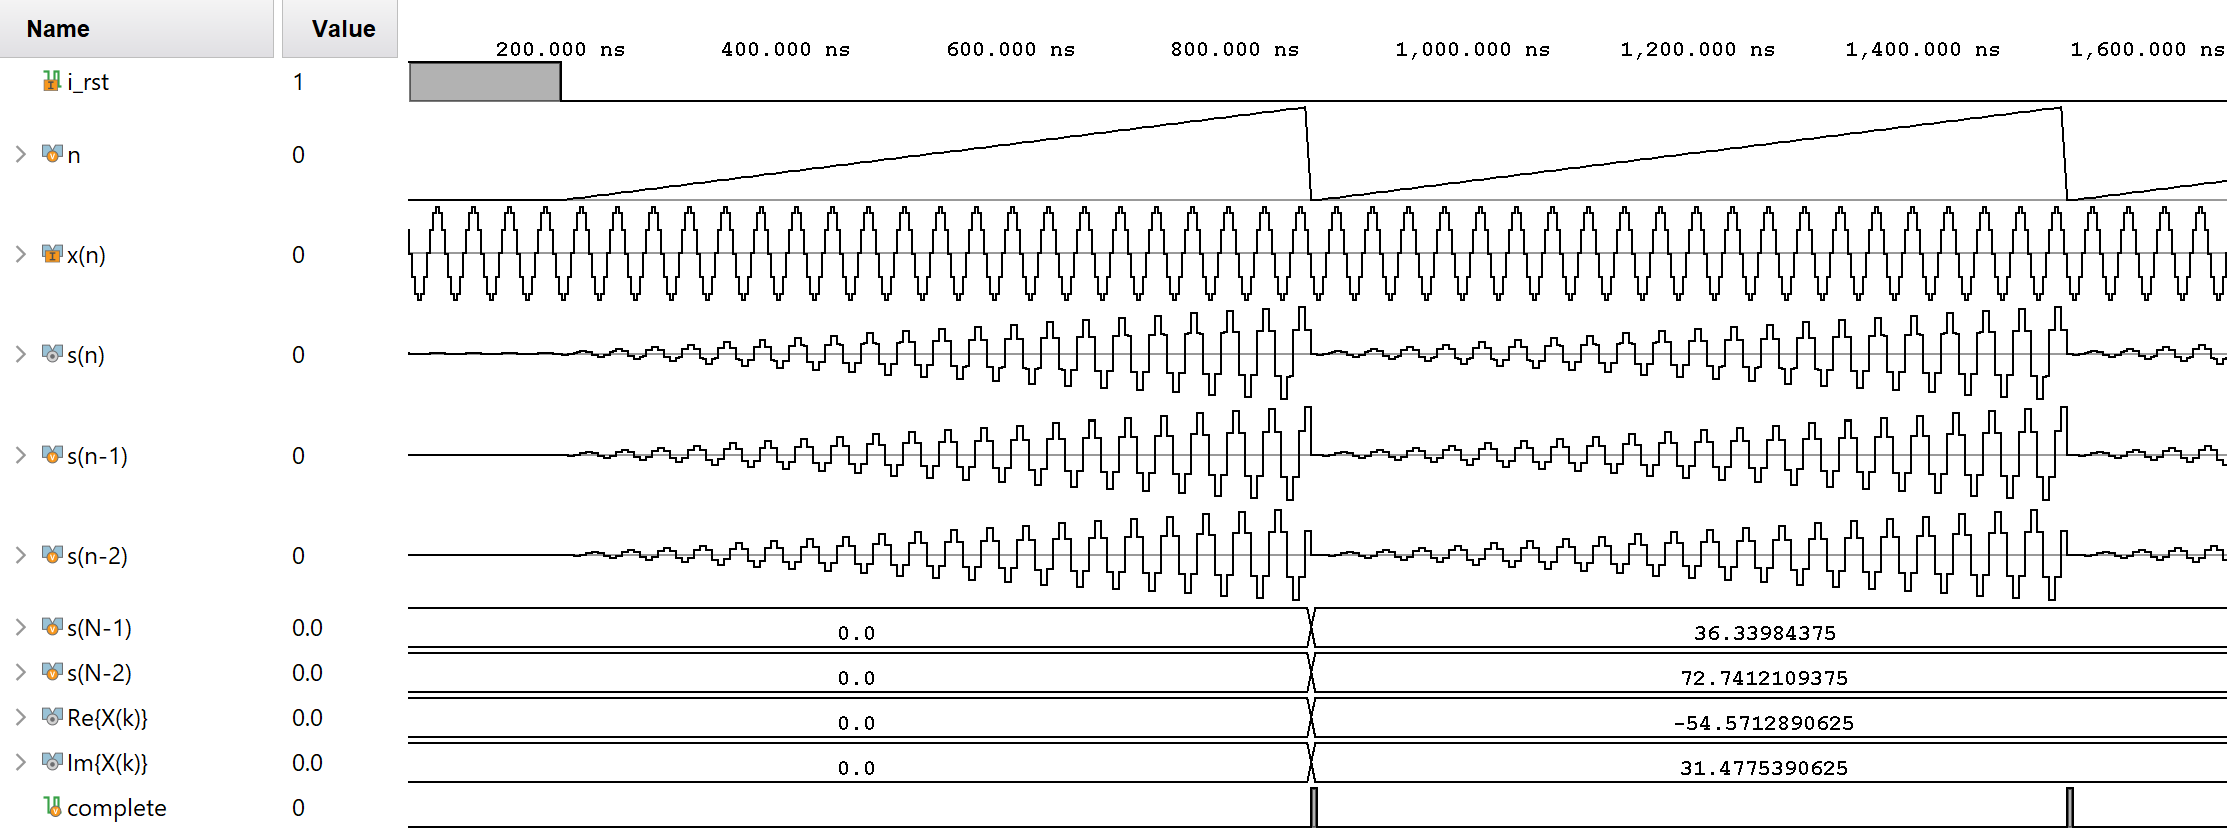
\includegraphics[width=\linewidth]{figs/goertzel_waveform0_inv.png}
    \caption{\textit{\textbf{Vivado}} generated waveform simulation for visualization of internal signal behavior of an example Goertzel filter within a testbench module.}
    \label{fig:15}
\end{figure*}

\section{Testing and Analysis}

\subsection{Simulation}

A common tool for testing designs is the \textit{testbench}. A testbench is simply a larger module which "encloses" the \textit{unit under test} (UUT), and helps to control the flow of the input and output for the module. Testbenches are most often used in conjunction with \textit{simulation}, in which software such as Vivado simulates the behavior of the design for verification prior to configuration of the device. Simulation serves as a much quicker method of analysis and debugging for a particular design as opposed to the laborious process of synthesis, design routing, design optimization, \textit{bitstream} generation, and PL configuration. See the appendix for details on the FPGA programming process.

The key analysis tool of the simulation environment within Vivado is the waveform window. This tool allows visualization of signals similarly to the depiction in \textbf{FIG. 10}, with time on the horizontal axis and signal value on the vertical axis. All internal and external signals of a design can be monitored for purposes of debugging and behavior verification.

In order to simulate an incoming signal, an external module instantiates the CORDIC algorithm which produces a 31.25 MHz, 12-bit signal. This simulated signal is nearly identical to what one might expect to see from an ADC, with the exception being that the sampling rate is limited to a single sample per clock cycle, and the signal is \textit{ideal}, meaning there is zero \textit{noise} in the data.

 Such waveform diagrams as the one in \textbf{FIG. 15} can appear intimidating, but close inspection will reveal important details necessary for understanding how the filter operates. Starting at the top of the diagram and working down, each wave corresponds with an internal signal (\verb+wire+ or \verb+register+) mentioned in the previous section concerning the implementation. For now, the clock and clock enable signal are ignored, since clock cycles are indistinguishable at the timescale of \textbf{FIG. 15}. 
 
 The first control signal, \verb+i_rst+, is externally controlled by the testbench. It provides a way of defining a "beginning" of the filtering process at its high-to-low transition.

 The next signal present is \verb+n+. This signal displays the counter tracking the sample number. Recall that at the very top of each cycle of the counter is when $n = N-1$, thus the falling edge of this waveform is precisely when each new conversion should be completed.

 The following signal, \verb|x(n)| is straightforward. It is the ideal, continuous wave input to the filter as externally generated by the CORDIC algorithm. As expected, it simply appears as a sine wave with constant, 12-bit signed amplitude (ranging from -2048 to 2047) at a frequency of 31.25 MHz.

 Recall the oscillatory behavior of the intermediate sequence depicted by \textbf{FIG. 9}. Represented in HDL as \verb|sum|, $s(n)$ elegantly displays the precise behavior we expect from C++ simulation---an oscillation with growing amplitude. Of course, $s(n-1)$ and $s(n-2)$ follow as identical waveforms to $s(n)$, but with one and two clock cycle delays, respectively. The delay is most easily observed by noting the signal values just before the internal reset at the end of each conversion.

 Next, $s(N-1)$ and $s(N-2)$, which are initialized to zeros and remain zero until the completion of the first conversion. Although some waveform magic was applied to display the values in fixed-point format (with 11 fractional bits, in this case), it's important to remember that these are stored in the registers as 20-bit signed integers.

 After the final combinatorial arithmetic is performed on $s(N-1)$ and $s(N-2)$, the real and imaginary components of $X(k)$ appear. They appear on the same clock cycle that $s(N-1)$ and $s(N-2)$ are obtained because the calculation is purely combinatorial.

 The final signal shown in \textbf{FIG. 15} is a simple control flag designed to go high for a single clock cycle after each conversion is complete. Such a flag can be used to tell connected modules when data is available to be read from the filter.

 In simulation, one might notice that the result is obtained once, but never changes even after successive conversions. This is an artifact of the ideal input signal. In a real-world scenario, slight variations in the signal facilitated by a noisy environment will produce a slightly different result after each conversion.

 In this particular instance of simulation, the filter gave a result, in A(8,11) format,
 \begin{align}
     \text{Re}\{X(k)\} & \simeq -54.6 \nonumber \\
     \text{Im}\{X(k)\} & \simeq 31.5 \nonumber \\ 
 \end{align}

 A simple magnitude calculation yields
 \begin{equation}
     |X(k)| \simeq 63.03
 \end{equation}

 Evidently, the imprecise fixed-point FPGA arithmetic introduces very little error into the final result on its own---less than $\frac{1}{20}$ of a percent!

\subsection{Development Boards}

Since experiments like \textit{CoRaLS} and \textit{PUEO} use highly specialized hardware, it is more feasible to use FPGA development boards to analyze the real-world performance of a design. \textit{Real Digital}'s RFSoC 4x2 Development Board provides plenty of features, including 4 ADC channels, 2 DAC channels, Ethernet, 8 GB of DDR4 RAM, an SD card slot for disk space, and support from the \textit{PYNQ} open-source Python framework.

In this case, the module represented in \textbf{FIG. 13} is only a small portion of a larger system of firmware for the 4x2 development board. Though the Goertzel filter is designed to be a "black box" that can be integrated with any larger system, the matter of getting data to and from the filter, as well as output handling, is dependent on the existing firmware and the chosen methods of handling discontinuities in filter output data, i.e. what happens when the continuous wave signal is no longer present according to the filter?

Once the filter module is behaving as expected in simulation, the RFSoC on the board must be configured properly. This process includes the programming, synchronization, and calibration of the board's clocks, memory, and ADCs in addition to the configuration of rest of the PL. The details here are board-specific (See Ref. \cite{github} for the GitHub managed Vivado project in its entirety).

In standard operation mode, the full-scale input of the ADCs is -0.5 V to +0.5 V (1 V amplitude), thus any analog signal within this range is properly converted without \textit{clipping}. A sine wave with an amplitude of 1 V should produce the expected value $|X(k)| = N/2 = 63$.

\subsection{PYNQ}

\begin{figure*}
    \centering
    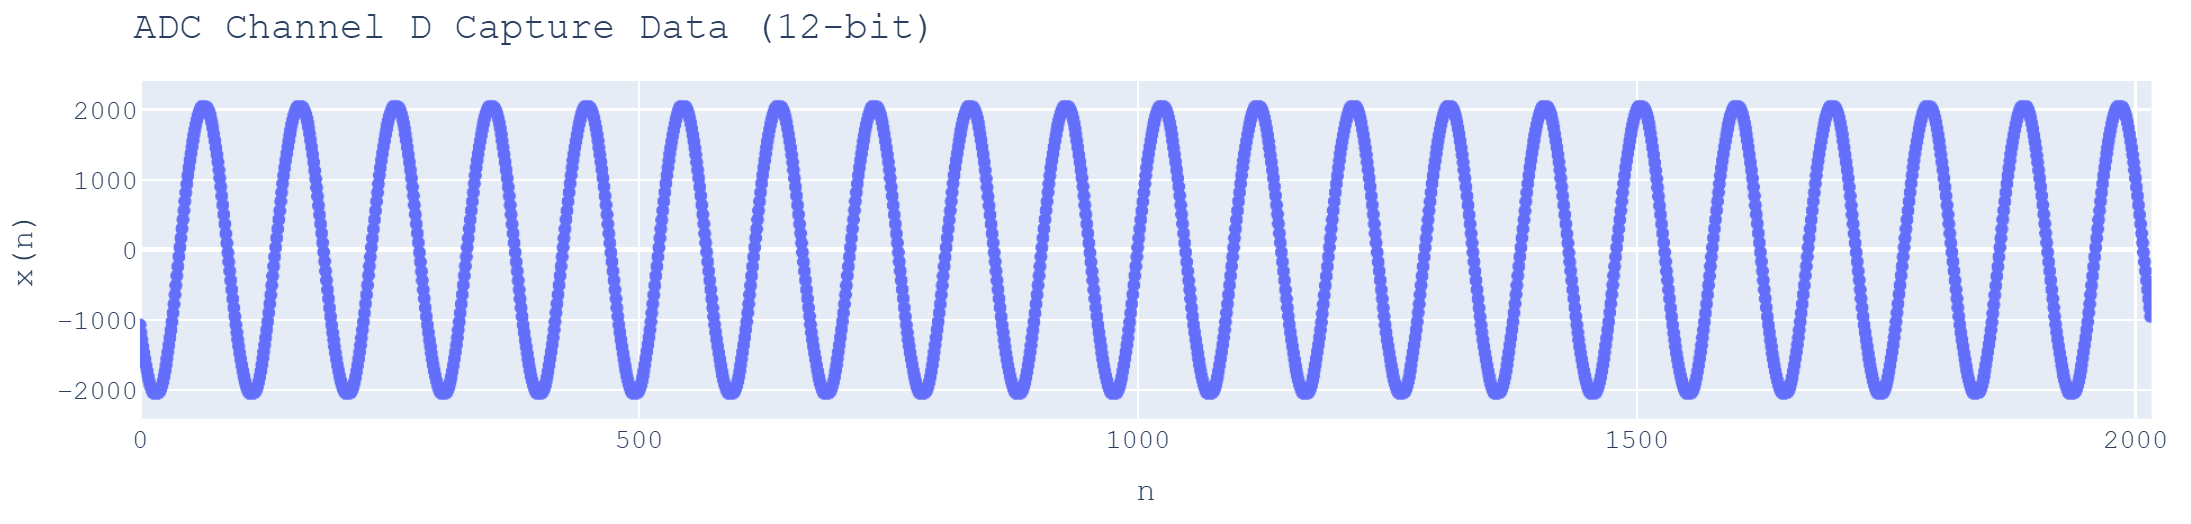
\includegraphics[width=\linewidth]{figs/ADC_data.png}
    \caption{ADC capture data read from the FPGA memory to an interactive Python kernel for plotting with a Jupyter notebook.}
    \label{fig:16}
\end{figure*}

\begin{figure}
    \centering
    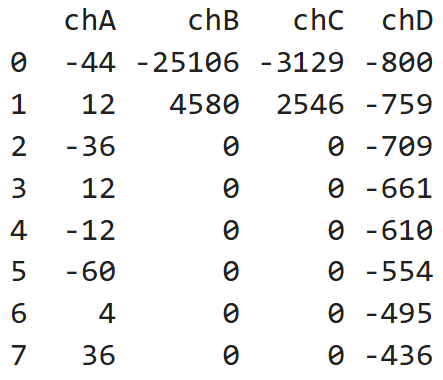
\includegraphics[width=0.8\linewidth]{figs/ADC_table.png}
    \caption{Raw data produced on each channel for a particular capture of 8 samples.}
    \label{fig:17}
\end{figure}

Once the necessary bitstream (\verb|.bit|) and hardware handoff (\verb|.hwh|) files have been generated by Vivado, the programmable logic of the physical FPGA is ready to be configured. For the 4x2 Development Board, an AMD-developed Python framework called \textit{PYNQ} supports this process.

PYNQ allows users to interface with the FPGA through the operating system on the board. Users access an instance of \textit{JupyterLab} through a browser on a separate machine with a USB or Ethernet connection to the board. From here, terminal commands, Python scripts, and Jupyter Notebooks can be created and executed directly on the processing system of the FPGA. This allows for direct manipulation of the file system and memory access as necessary for configuration and testing of the FPGA design. After uploading the bitstream and hardware handoff file to the file system in JupyterLab, a Python class of the PYNQ framework---an \verb|Overlay|---is instantiated, which initiates the process of configuring the programmable logic with the data from these files.

For confirmation that PYNQ is working properly, the initial design is set up such that output from all four ADC channels are sent directly to memory using four \textit{ADC capture} modules (\verb|adc_cap_x2.v|) so that the interactive Python kernel can access and manipulate the data. 

Using an external function generator (\textit{Hewlett-Packard 8665B}), a 31.25 MHz analog signal is passed directly to the SMA connector of the board on channel D. The data is read and plotted using Python as shown in \textbf{FIG. 16}. The continuous wave appears, with a value that ranges from -2048 to 2047 as expected. There is little control over the exact instant that the ADC memory is read, so the phase of the wave in \textbf{FIG. 16} is randomized.

\subsection{Firmware Details}

Remember, for every clock cycle of the 375 MHz system clock on the FPGA, the ADCs each produce eight samples. While the ADCs are technically only accurate to 12 bits, the raw data samples are actually 16 bits each. In firmware, this means that each data channel from ADC to memory is 128 bits wide in order to hold eight 16-bit samples per clock cycle.

In order to see the results from the Goertzel filter in memory, the filter overrides a second ADC channel (channel C) to pass along the filtered data from channel D. By truncating the output of the filter down to two 16-bit values for Re$\{X(k)\}$ and Im$\{X(k)\}$, each component then takes up the same space as one sample in the data stream. The overridden channel data produces the Goertzel filter output as the first and second sample out of every eight. A capture of eight sequential samples produces a table like the one in \textbf{FIG. 17}. The remaining samples are filled with zeros. The values in channel A and B strictly reflect the measurement of thermal noise within the environment.

Plotting the data for channel C similarly to channel D would look like nonsense. Instead, Goertzel output data should be acquired 8 samples at a time, yielding 16-bit integer forms of Re$\{X(k)\}$ and Im$\{X(k)\}$ as the first two samples only. Recall from the Vivado simulation that results were produced in fixed-point form, A(8,11). This was before truncation when each component was stored as a 20-bit integer. To get down to 16 bits, the bottom four fractional bits were dropped. Each pair of integers on channel C must be in A(8,7) format. To get $X(k)$, perform the following conversion:
\begin{lstlisting}[language=Python]
    Xk_re = chC[1] / 2**7
    Xk_im = chC[0] / 2**7
\end{lstlisting}
Calculating the magnitude is a trivial extra step in Python. For the values in the table of \textbf{FIG. 17}, the result is not too far off from expectations, yielding
\begin{equation}
    |X(k)| \simeq 63.42
\end{equation}
As expected, noise does affect the result. In this case, the relative error is 0.007 (0.7\%).

\begin{figure*}
    \centering
    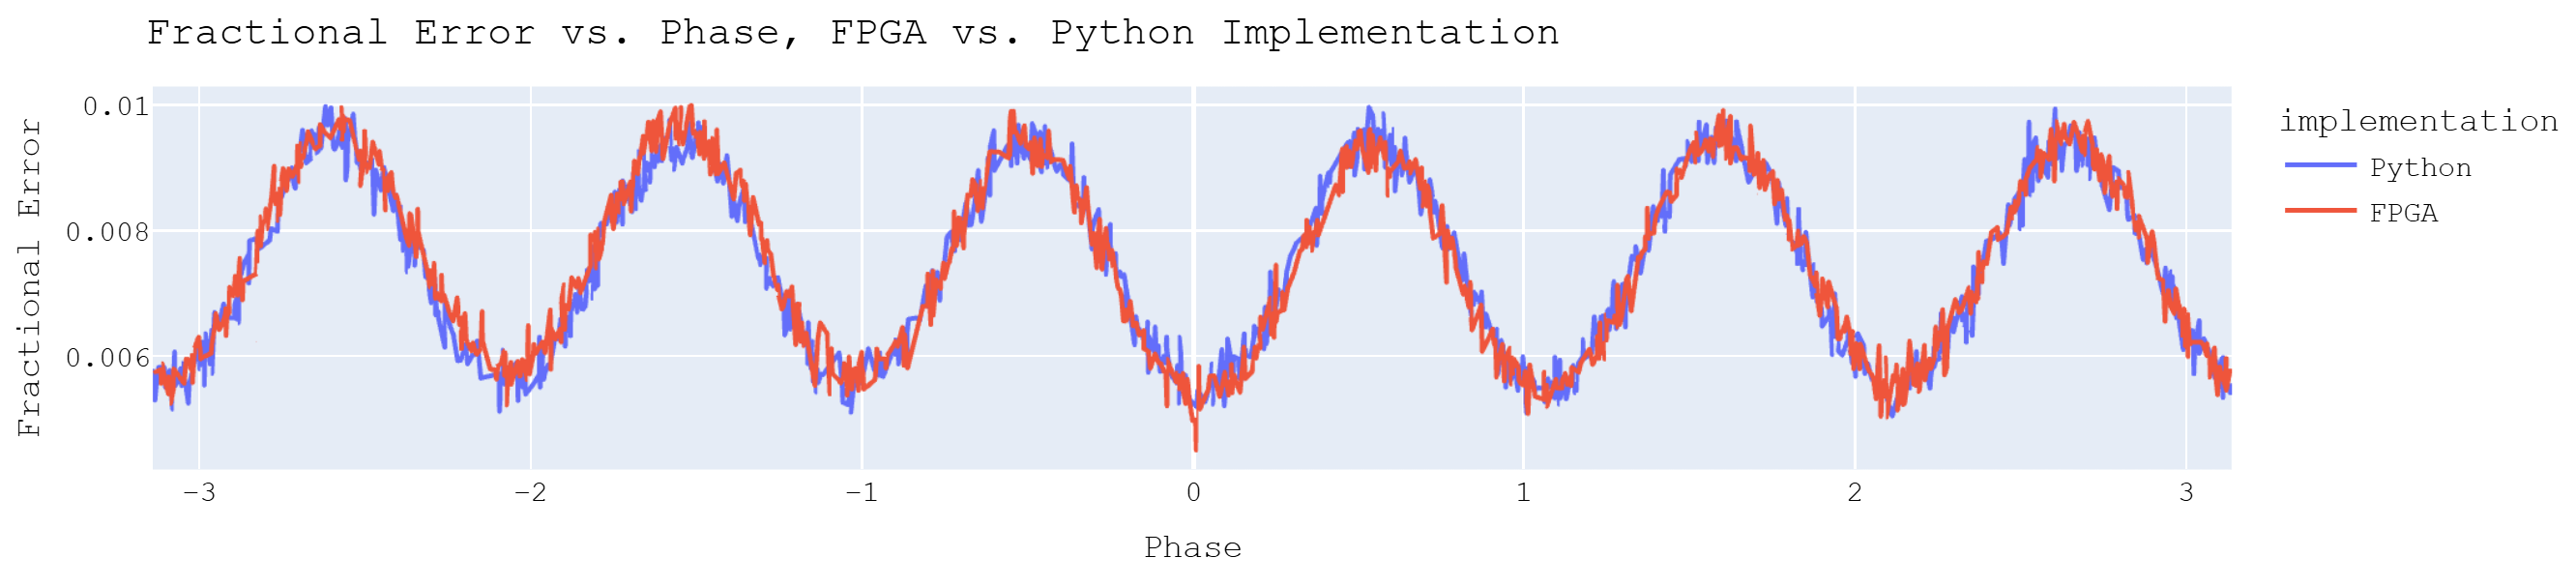
\includegraphics[width=\linewidth]{figs/pythonvfpga.png}
    \caption{Fractional error produced by the FPGA implementation of the filter compared with a Python implementation to illustrate the systematic error introduced by fixed-point arithmetic. The horizontal axis shows the phase of each filter output for 1000 iterations.}
    \label{fig:18}
\end{figure*}

\begin{figure}
    \centering
    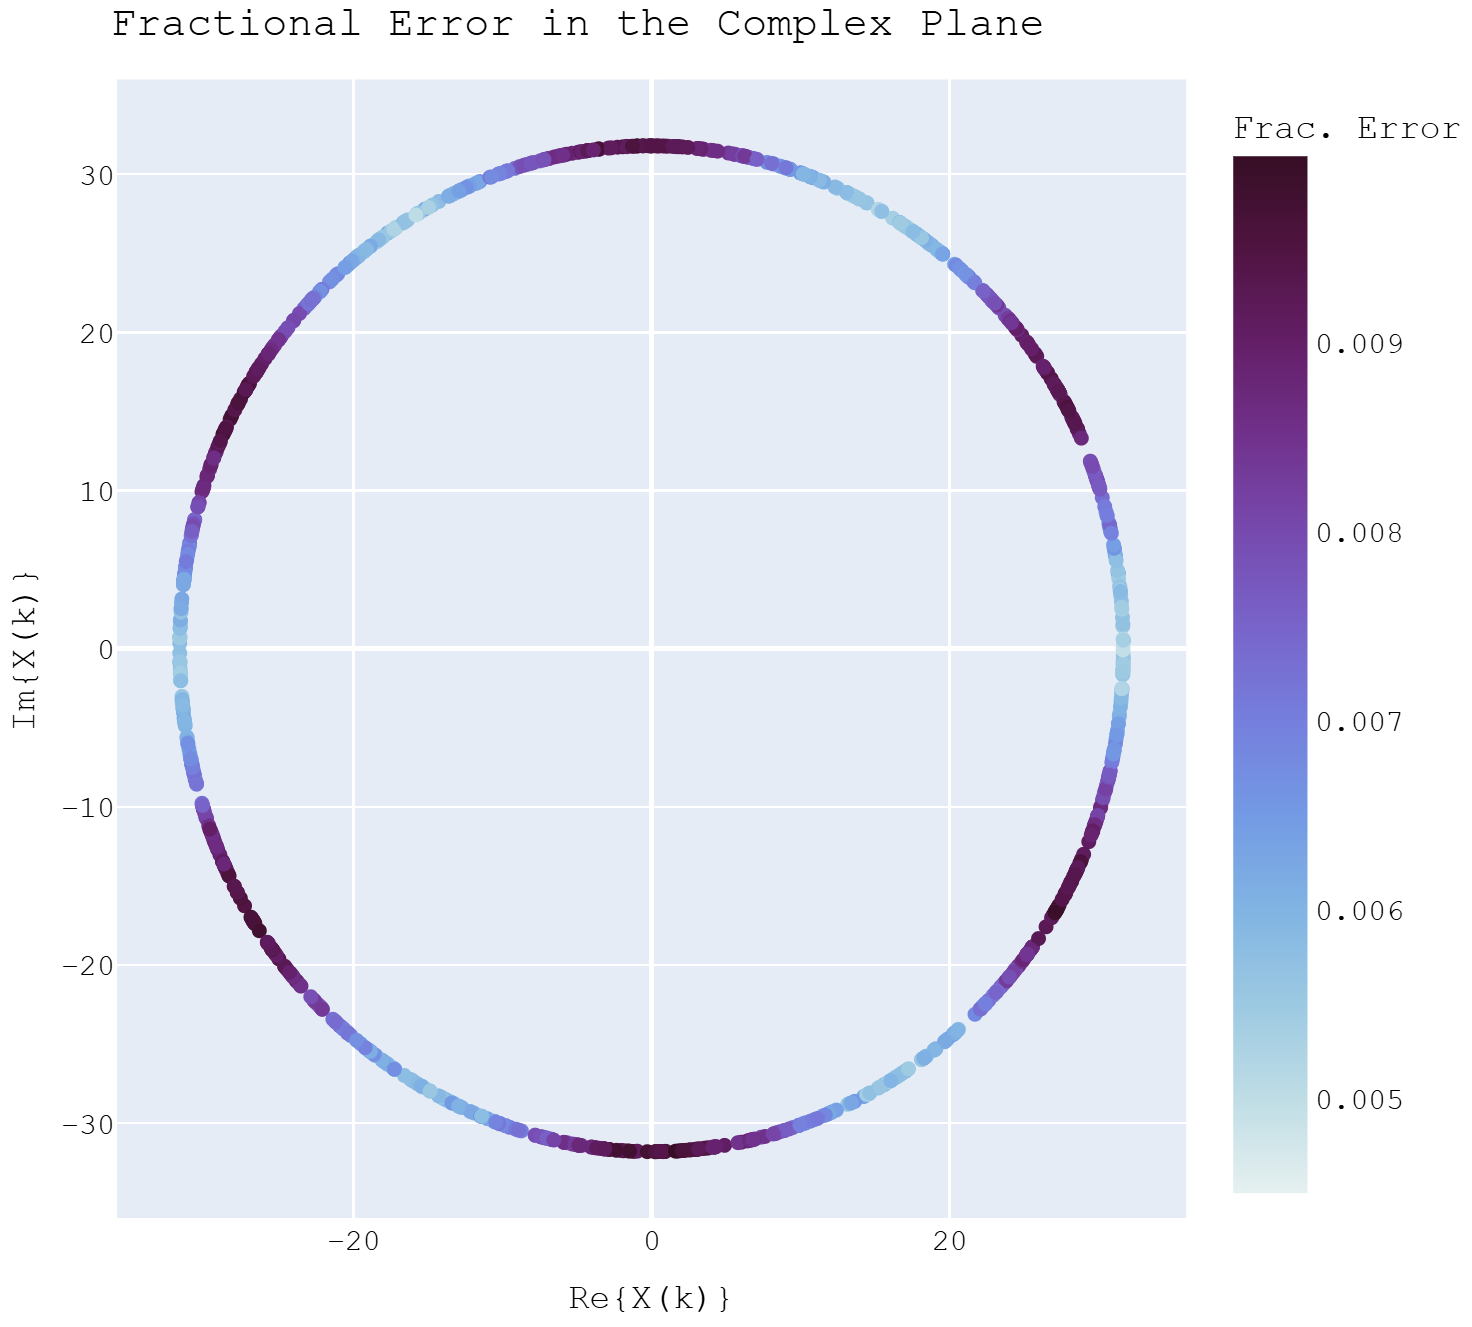
\includegraphics[width=\linewidth]{figs/error_complex.png}
    \caption{Complex plane plot of 1000 consecutively obtained values for X(k) according to the firmware implementation of the Goertzel filter in a low-noise environment. This error is fractional, not a percentage.}
    \label{fig:19}
\end{figure}

\subsection{Error Analysis}

In simulation, the generated waveform was not only noiseless, but also \textit{phase-locked}. The phase of the input and output never changed or "walked" out of alignment with the system clock, because the input itself was derived from the system clock. Because the function generator has not been explicitly phase-locked with the clock on the FPGA, the signal fed to the algorithm is likely to shift in and out of phase alignment. On the time scales of acquiring the values in PYNQ, this phase shift can be quite significant. For example, an difference in the signal period of one part in a million (\textit{difference} meaning variation from what the FPGA "thinks" is 31.25 MHz) would result in a full cycle delay after only a million cycles, which occurs quite quickly ($\sim 32$ ms) at this frequency.

In short, the function generator cannot produce a 31.25 MHz signal precisely in the FPGA clock domain. Because of the resulting "phase walk", non-consecutive acquisitions of the filter output are almost guaranteed to result in values with a completely randomized phase. Taking advantage of this, 1000 iterations of acquiring output and plotting produces \textbf{FIG. 18} and \textbf{19}. \textbf{FIG. 19} shows all 1000 values in the complex plane, with a color corresponding to the fractional error, $\epsilon$, of the magnitude from the expected value.

\begin{equation}
    \epsilon = \frac{A_k - \langle A_k \rangle}{\langle A_k \rangle}
\end{equation}
where $A_k = |X(k)|$. Plotting $\epsilon$ against the phase produces \textbf{FIG. 18}. Alongside the results produced by the FPGA implementation of the filter (in red) are 1000 results obtained by a Python implementation of the filter (in blue) which also took ADC data as input.

Because the FPGA implementation closely matches the Python implementation, it would seem that the systematic error introduced by fixed-point arithmetic can essentially be ignored.

Clearly, the error is a sinusoidal function in phase-space as shown in \textbf{FIG. 18}. For a 187.5 MHz sample rate of a 31.25 MHz signal, each period corresponds to exactly six samples. The low points in the plot represent the phase values at which the generated signal is "correctly" aligned within the clock domain of the FPGA. In the interest of minimizing error for a real-world application, phase-locking between the signal and the FPGA clock domain is desirable, such that the phase of the filter input and output can be controlled.

An analog sinusoid with an amplitude of 1 V actually ranges from -0.5 V to +0.5 V, which is converted to a 12-bit digital signal ranging from $-2^{11}$ to $2^{11} - 1$. The magnitude of the filter output is linearly dependent on this signal amplitude,
\begin{equation}
    |X(k)| = \frac{N}{2}A
\end{equation}
where A is the amplitude of the signal (in units of volts). 

As a result, the \textit{vertical shift} of the error in phase-space is also linearly dependent on the amplitude, $A$. In fact, since the definition of $\epsilon$ has no absolute value in the numerator, the fractional error, $\epsilon$, can go negative. The precision of the filter then partially relies on the precision of the instrumentation in generating a wave that has the correct amplitude once it reaches the ADCs. This might be a trivial conclusion, but in practice it can be used to finely tune the system such that $|X(k)|$ oscillates around a specified value without too much concern for phase-locking.

\section{SNR and Frequency Response}

How might the filter respond if there is significant variation in the frequency of the controlled external signal? In what frequency range will the single component still be "detected"?

Returning to C++ simulation methods, plotting $|X(k)|$ over a range of frequencies results in a "pseudo-frequency response" for the filter, shown in \textbf{FIG. 20}. 

\begin{figure}[H]
    \centering
    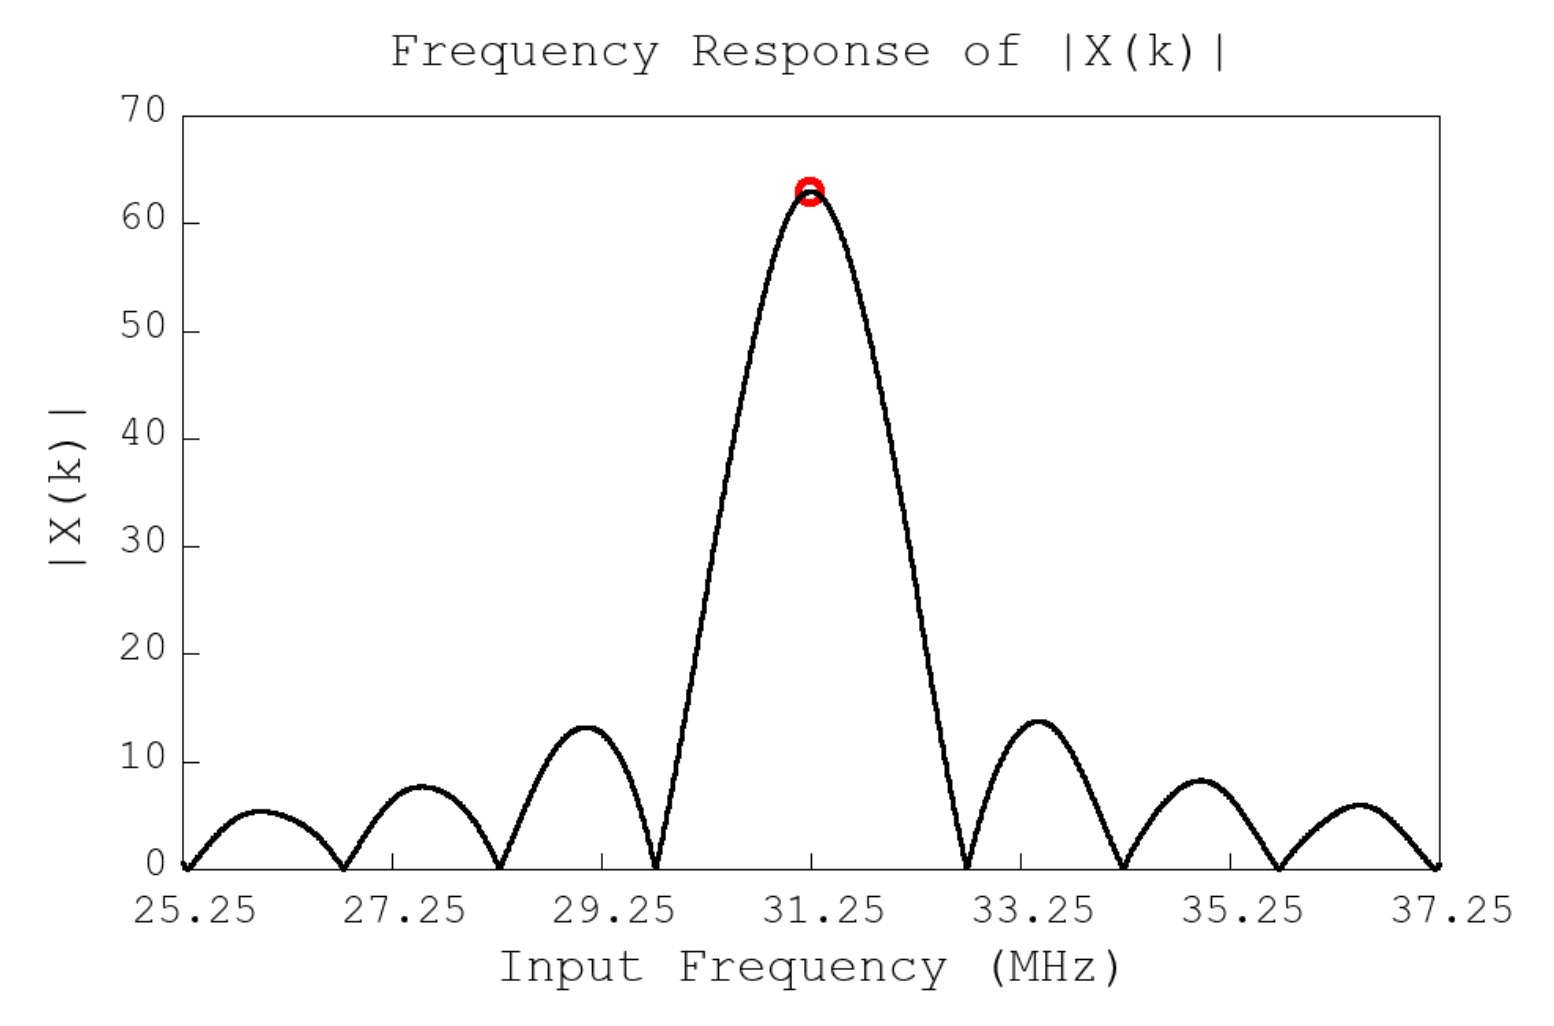
\includegraphics[width=\linewidth]{figs/frequency_response.png}
    \caption{\textit{Pseudo}-frequency response of the filter, generated with C++ by plotting the $|X(k)|$ output of the filter over a range of frequencies around the target frequency. The red dot marks the precise location of $f = 31.25$ MHz and $|X(k)| = 63$.}
    \label{fig:20}
\end{figure}

It's important to understand the response of a filter in the presence of increased noise. One method of characterizing the presence of noise is the \textit{signal-to-noise ratio} (SNR). In units of decibels (dB), the SNR is given by
\begin{equation}
\text{SNR}_{\text{dB}} = 10 \log_{10}\left( \frac{P_{\text{signal}}}{P_{\text{noise}}} \right)
\end{equation}
where P is the power (See Ref. \cite{Johnson:2006:SNR}). Defining power can be a bit tricky, but generally, for a discrete signal the power is given by the mean square value of the signal.
\begin{equation}
    P = \langle s^2 \rangle = \frac{1}{N} \sum_{n=0}^N s^2(n)
\end{equation}

\begin{acknowledgments}
    \blindtext
\end{acknowledgments}

\appendix

\section{The AXI4-Stream Interface}

The AXI4-Stream interface is ...

\blindtext

\section{FPGA Configuration Process}

Configuring FPGAs...

\blindtext

\section{The CORDIC Algorithm}

In simulation...

\blindtext

\nocite{*}
\bibliography{sources}% Produces the bibliography via BibTeX.

\end{document}
%
% ****** End of file apssamp.tex ******
